\chapter{Network}\label{chap:network}
This chapter considers interactions between multiple stakeholders in mobile networks and studies the resulting tradeoffs.
These tradeoffs have only appeared recently with the advent of smartphones.
With traditional cell phones, traffic in networks was largely dominated by voice traffic and to a smaller degree by text and signalling messages.
%So called feature phones introduced, together with the concept of mobile applications, new types of traffic.
%Here, mostly web traffic and, to a lesser extend, traffic generated by applications occurred.
%However, applications were either proprietary and designed by phone vendors or did not find widespread adoption, so that the generated traffic had little impact on the mobile network.
The introduction of smartphones resulted in an increased amount of applications, developed by a decentralized developer community.
With the application ecosystem no longer being under control of network operators, as in the case of voice or text messages, or hardware vendors, as with the rudamentary bundled applications of early feature phones, new types of network traffic occured and replaced voice and signalling as the main traffic type.
% centralized network management and end-to-end traffic engineering became difficult for network operators.
Furthermore, the amount of traffic is no longer the only performance indicator for the network operator, and the network operator is no longer the only stakeholder involved in the mobile network ecosystem.

\begin{figure}
  \centering
  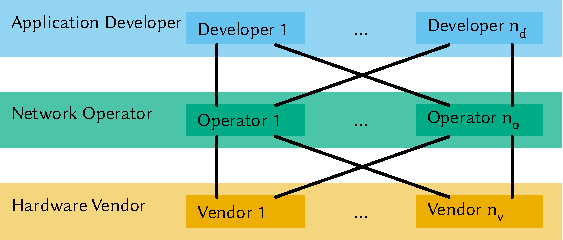
\includegraphics{network/figures/stakeholders}
  \caption{Stakeholders investigated in the network scenarios}
  \label{fig:network:stakeholders}
\end{figure}

Each of the stakeholders shown in \reffig{fig:network:stakeholders} is interested in optimising the network, device, or application performance in order to improve relevant \glspl{KPI}.
To this end, each of the stakeholders can manipulate the parts of the network that it controls.
The \emph{network operator} can change network configuration parameters in order to reduce \emph{signalling} in the network.
Hardware \emph{vendors} can configure smartphones in such a way that data connections are terminated as soon as possible, decreasing \emph{power drain}.
\emph{Application developers} can increase polling intervals in their application layer protocols in order to increase \emph{\gls{QoE}}.	
However, the parameters the stakeholders can influence in order to optimise the \gls{KPI} of their individual concerns, also influences the complete network and thus all other \glspl{KPI}, possible to the detriment of the other stakeholders.
When a stakeholder attempts to optimise \glspl{KPI} of interest, the consequences for other stakeholders have to be considered, as they could consider optimising their respective \glspl{KPI} in turn, resulting in a net loss for all participating stakeholders.
Thus, a tradeoff between all considered \glspl{KPI} is required in order to satisfy the participating stakeholders.

Current best practices result in each participant optimising the respective \glspl{KPI} individually, without adressing the needs of the other stakeholders~\cite{Qian2011a,NSN2011}.

The contribution of this chapter is threefold:
\begin{enumerate*}
\item We provide an algorithm to infer metrics for the relevant \glspl{KPI} for the stakeholders from traffic traces, and evaluate exemplary traces for a set of popular applications.
\item We develop an analytic model in order to analyse theoretical and empirical application traffic distributions and derive \glspl{KPI} for the stakeholders.
\item We study the impact of network timer optimisation, a practice where network operators modify network parameters in order to optimise signalling unilaterally, and show the impact for other stakeholders and highlight potential consequences for the network operator.
\end{enumerate*}

The content of this chapter is taken from~\cite{Schwartz2013a,Schwartz2013c}.
Its remainder is structured as follows.
First, we give a background of mobile networks and survey related work in \refsec{sec:network:background}.
In \refsec{sec:network:network_traces}, we perform application traffic measurements and investigate the impact of application traffic on \gls{UE} power drain, network signalling and web \gls{QoE} for a selected set of applications.
Then, we generalize our results by introducing an analytic model in order to derive metrics for state transition frequency and power drain from arbitrary traffic distributions in \refsec{sec:network:performance_model}.
Finally, we conclude this chapter with lessons learned in \refsec{sec:network:lessons_learned}.

\section{Background and Related Work}\label{sec:network:background}
This section discusses the technical background relevant to the remainder of this chapter.
First, in \refsec{sec:network:background:umts_rrc} we introduce the \gls{UMTS} mobile communication standard, and the \gls{RRC} protocol.
Then we discuss existing aproaches to measure \gls{RRC} protocol transactions and optimise the signalling load generated by \gls{RRC} messages in \refsec{sec:network:background:measurement_optimisation}.
Finally, \refsec{sec:network:background:energy_consumption_qoe} tackles smartphone power consumption and \gls{QoE}, two metrics influenced by the configuration of the \gls{RRC} protocol.

\subsection{\headershortacr{UMTS} Networks and the \headershortacr{RRC} Protocol}\label{sec:network:background:umts_rrc}
A \gls{3G} \gls{UMTS} mobile network consists of three main components, which are depicted in \reffig{fig:network:background:mobile_network_overview}: The \gls{UE}, the \gls{RAN}, and the \gls{CN}.
The \gls{RAN} is used to establish connectivity between the \gls{UE} and the \gls{CN}, which in turn can establish connectivity to the Internet, if required.

\begin{figure}
	\centering
	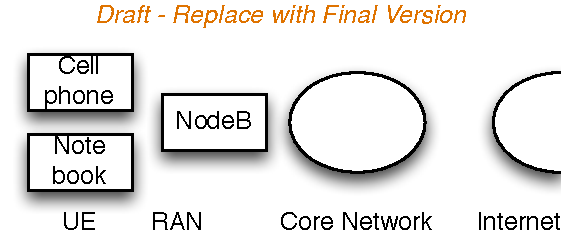
\includegraphics{network/background/figures/mobile_network_overview}
	\caption{Overview of Mobile Network}
	\label{fig:network:background:mobile_network_overview}
\end{figure}

\gls{UE} consists of devices used by end users, i.e. smartphones, tablets or data card enabled notebooks, but can also include \gls{M2M} devices.
The \gls{RAN} is, amongst other tasks, responsible for \gls{RRC}, packet scheduling and handover control.
It includes network entities such as the \gls{NodeB} and the \gls{RNC}.
The \gls{CN} provides the backbone network of the \gls{UMTS} network and provides connectivity to the Internet and the \gls{PSTN}.
Furthermore, functionality such as billing, authentication and location management is provided by the \gls{CN}.

In UMTS networks, the radio resources in the RAN between base station and UE are controlled and managed by the \gls{RRC} protocol~\cite{3GPP_RRC_Spec}.
The protocol offers services such as broadcast of network information, maintenance of a connection between the \gls{UE} and \gls{RAN}, establishment of point-to-point radio bearers for data transmission, \gls{QoS} control, and reporting and cell selection management.
The protocol is divided into different parts: services for upper layers, communication with lower layers, protocol states, \gls{RRC} procedures, and error control.
In particular, \gls{RRC} also participates in the co-ordination of other resource management operations such as channel measurements and handovers.
All \gls{RRC} procedures rely on protocol states which are defined to trigger action should be applied and which information must be signaled. 
The state are defined per \gls{UE} and for the connection between the \gls{UE} and the \gls{NodeB} station.
Typically there are five \gls{RRC} states characterizing a connection between \gls{UE} and \gls{NodeB}: \texttt{idle}, \texttt{URA\_PCH}, \texttt{CELL\_PCH}, \texttt{RRC\_DCH}, and \texttt{RRC\_FACH}.
Whether a specific \gls{RRC} state is used in a specific mobile network depends on the configuration of the network by the provider.
In the following we concentrate on the most commonly observed~\cite{Qian2010a} \gls{RRC} states \gls{RRC_idle}, \gls{RRC_DCH}, and \gls{RRC_FACH}.
We neglect \texttt{URA\_PCH} and \texttt{CELL\_PCH} in this study.
While \texttt{URA\_PCH} plays only a role in scenarios of high mobility, \texttt{CELL\_PCH} is not yet widely implemented. 
Our results are still of general nature and do not depend on the limited number of considered \gls{RRC} states.

If the \gls{UE} is switched on and no connection to the mobile network is established, the \gls{UE} is in \gls{RRC_idle} state.
If the \gls{UE} wants to send data, radio resources are allocated by the \gls{NodeB} for the handset and the \gls{UE} will transition to either the \gls{RRC_FACH} or the \gls{RRC_DCH} state. 
Then, a corresponding channel for data transmission is assigned to the \gls{UE}.
The \gls{RRC_FACH} and the \gls{RRC_DCH} state can be distinguished in that way that in \gls{RRC_DCH} state a high-power dedicated channel for high speed transmission is allocated whereas in \gls{RRC_FACH} state a shared access channel for general sporadic data transmission is used.
Thus, \gls{RRC_FACH} consumes significantly less power than the \gls{RRC_DCH} state. 

The possible transitions between the different states are defined by the network operator and the \gls{RRC} protocol stack.
Typically, the following state transitions are included: 
\gls{RRC_idle} \(\rightarrow\) \gls{RRC_FACH},
\gls{RRC_FACH} \(\rightarrow\) \gls{RRC_DCH} to switch from lower radio resource utilization and low \gls{UE} energy consumption to another state using more resources and energy, and 
\gls{RRC_DCH} \(\rightarrow\) \gls{RRC_FACH}, 
\gls{RRC_FACH} \(\rightarrow\) \gls{RRC_idle},
\gls{RRC_DCH} \(\rightarrow\) \gls{RRC_idle} to switch to lower resource usage and energy consumption.
According to~\cite{Perala2009,Qian2010a}, the transitions are triggered by user activity and radio link control buffer level. 
A transition from \gls{RRC_DCH} to \gls{RRC_FACH} usually occurs when the buffer is empty and a threshold for a release timer is exceeded, resulting into the corresponding \gls{RRC} protocol message flow.
A transition in the reverse direction is triggered if the buffer level exceeds a specified threshold value for a predefined time period.
The \gls{UE} will transition into \gls{RRC_idle} state if the \gls{RNC} detects overload in the network or no data was sent by the \gls{UE} for a specified time.

\begin{figure}
	\begin{subfigure}[b]{.5\textwidth}
	\centering
	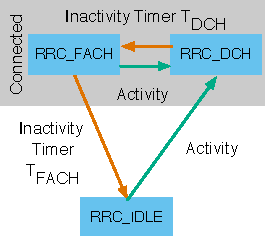
\includegraphics{network/background/figures/three_states}
	\caption{Three State Scenario}\label{fig:network:background:rrc_state_machines:three_states}
	\end{subfigure}
	\begin{subfigure}[b]{.5\textwidth}
	\centering
	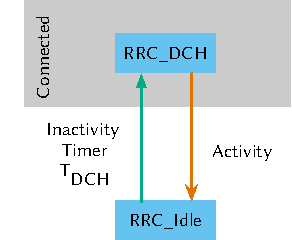
\includegraphics{network/background/figures/two_states}
	\caption{Two State Scenario}\label{fig:network:background:rrc_state_machines:two_states}
	\end{subfigure}
	\caption{\headershortacr{RRC} State Machine Diagrams}\label{fig:network:background:rrc_state_machines}
\end{figure}

In the following, we consider two different state transition models, depicted in \reffig{fig:network:background:rrc_state_machines}, based on the \gls{RRC} protocol.
The first model includes the \gls{RRC_idle}, \gls{RRC_FACH}, and \gls{RRC_DCH} states is shown in \reffig{fig:network:background:rrc_state_machines:three_states} and is in the following called the three state model.
If the \gls{UE} is in the \gls{RRC_idle} state and activity is detected, i.e. a packet is sent or received, the connection transitions to \gls{RRC_DCH} state.
After each transmission a timer \gls{TDCH} is started and reset whenever a new packet is sent or received.
If the timer expires, the connection transitions to the \gls{RRC_FACH} state
Upon entering, the \gls{TFACH} timer is started.
If a new transmission occurs, the connection again transitions to the \gls{RRC_DCH} state.
If \gls{TFACH} expires, the connection transitions to \gls{RRC_idle} state.

The second model, denoted as the two state model, and shown in \reffig{fig:network:background:rrc_state_machines:two_states}, only includes the \gls{RRC_idle} and \gls{RRC_DCH} state.
If the \gls{UE} is in the \gls{RRC_idle} mode and a packet is sent or received, the connection transitions to the \gls{RRC_DCH} state. Once in \gls{RRC_DCH} mode, the \gls{TDCH} timer is started and it is reset whenever a new packet is sent or received.
If the timer expires, the \gls{UE} transitions back to \gls{RRC_idle} state.

While the three state model is closer to the specified \gls{RRC} protocol is similar to some proprietary \emph{Fast Dormancy} implementations used by \gls{UE} vendors.
In these Fast Dormancy implementations, the \gls{UE} tears down the connection to the network state as soon as no data is ready to be sent for a certain time, i.e., it forces the network to transition to \gls{RRC_idle} state.
In contrast to the three state model, there is no transition to the \gls{RRC_FACH} state.
If a device disconnects from the network by transitioning to the \gls{RRC_idle} state, it has to be reauthenticated before another transition to the \gls{RRC_DCH} state can occur.
This results in additional signalling traffic and causes more load on the network \cite{NSN2011} due to frequent re-establishments of the RRC connection.
These proprietary Fast Dormancy algorithms do not adhere to the \gls{RRC} specification \cite{GSM2010}, but nontheless exist in the real world and have been identified as possible causes for signalling storms.
The major reason for Fast Dormancy implementations is the decrease in power consumption on the \gls{UE}, since the transmission unit of the \gls{UE} consumes only \SIrange{1}{2}{\percent} of the energy in \gls{RRC_idle} state compared to the \gls{RRC_DCH} state.
Thus, both models warrant further investigation.

\subsection{Measurements of \headershortacr{RRC} Parameters and Optimisation of Resource Consumption}\label{sec:network:background:measurement_optimisation}

In the literature, the configuration of the inactivity timers used for the \gls{RRC} protocols have been investigated in detail.
In~\cite{Perala2009} a measurement tool for \gls{RRC} protocol states is presented. 
It is used to determine \gls{RRC} state transition parameters, channel setup delays, and paging delay by measuring the one-way round trip time of data packets.
The results are validated by monitoring the energy consumption in different \gls{RRC} states.
One outcome is that \gls{UMTS} network configurations vary significantly by network operator.
\gls{RRC_DCH} release timer as well as the inactivity timer value triggering transition to \gls{RRC_idle} state were measured.
The values range from \SI{1.2}{\second} for the \gls{RRC_DCH} release timer to more than one minute for the \gls{RRC_idle} timer.
Similar results are presented in~\cite{Qian2010a}.
Here, the observed values vary between \SI{5}{\second} and \SI{12}{\second}. 
Additionally, they also determined the exact \gls{RRC} state transitions for two networks such as \gls{RRC_idle} \(\rightarrow\) \gls{RRC_FACH} \(\rightarrow\) \gls{RRC_DCH} or \gls{RRC_idle} \(\rightarrow\) \gls{RRC_DCH} directly without transitioning through the \gls{RRC_FACH} state.
The \gls{3GPP} has released a technical report \cite{3GPP_22801} about the adverse impact of mobile data applications.
This report states that frequent connection re-establishments due to small data packets caused e.g. by status updates of social network or instant messaging apps can lead to problems of increased signalling load.
This highlights the importance of this topic.

Furthermore, there are papers that propose optimizing strategies that take the \gls{RRC} states into account. 
In~\cite{Qian2011} the impact of different application traffic patterns is studied to reveal resource usage in mobile networks.
By identifying packet bursts, they infer the \gls{RRC} states of the \gls{UE}.
Radio resources are quantified by channel occupation time and energy consumption.
They propose an algorithm that tries to optimize application traffic patterns by e.g. piggybacking, batching up data, or decreasing the update rate of an application.
The algorithm is evaluated for six applications, two news applications, Pandora streaming application, Google search, Tune-In radio and Mobelix. 
In~\cite{Qian2010b} also \gls{RRC} states are studied for network optimization.
The authors optimize the inactivity timers to allow a better resource utilization. 
They propose a application-to-network interface to avoid unnecessary timer periods after data transmission.

\subsection{Smartphone Power Consumption and \headershortacr{QoE}}\label{sec:network:background:energy_consumption_qoe}
Power consumption of the \gls{UE} varies according to the devices current \gls{RRC} state.
The power consumption caused by \gls{RRC_DCH} mode was measured at about \SIrange{600}{800}{\milli\watt}~\cite{Qian2011,Qian2010a}.
In \gls{RRC_FACH} mode, the consumption was measured at about \SIrange{400}{460}{\milli\watt} depending on the \gls{UE} and the network operator~\cite{Qian2010a}.
A precise measurement of the power consumption of different \gls{RRC} states is performed in~\cite{Qian2010a,Balasubramanian2009,Lee2004}. 
The authors report that the energy drain depends on two factors: 
\begin{enumerate*}
\item user interactions and applications 
\item platform hardware and software.
\end{enumerate*}

In \cite{Ickin2012} the authors performed a 4 week long study with 29 participants to identify factors influencing \gls{QoE} of mobile applications.
The study comprises
\begin{enumerate*}
\item data from context sensing software,
\item user feedback using an experience sampling method several times per day, and
\item weekly interviews of the participants.
\end{enumerate*}
To determine the factors of influence, the authors analyze the frequency of specific keywords in the interviews and the surveys.
They find that the term \emph{battery} has the highest frequency.
According to the authors this is reasonable since the battery efficiency has a strong impact on the user perceived quality, in particular when it the \gls{UE} is nearly discharged.
\section{Inferring Signalling Frequency and Power Consumption from Network Traces}\label{sec:network:network_traces}
All participating stakeholders, i.e. network operators, hardware vendors, and application developers, need to assess the impact of potential changes of parts of the mobile network, e.g. change of network parameters, introduction of new hardware or modification of applications, on their considered \glspl{KPI} without rolling out changes to the production network.
To this end, we propose specific metrics in order to quantify the impact of changes on the network on the considered \gls{KPI}.
We introduce an algorithm to infer metrics from application traffic measurements, network parameters and power and signalling configurations.
In \refsec{sec:network:network_traces:performance_evaluation} we present the algorithm and methods to describe the relevant metrics.
Then, in \refsec{sec:network:network_traces:numerical_results}, we use the proposed methodology to evaluate the impact of various network configurations on four popular applications.

\subsection{Inferring State Transitions and Deriving Metrics}\label{sec:network:network_traces:performance_evaluation}
A \gls{UE}’s firmware triggers \gls{RRC} state transitions based on application traffic.
While solutions exist to capture RRC state transitions on specific hardware~\cite{zayas2010} they are not available for all modern smartphone platforms.
Other options to measure the required information include using costly hardware and use specific \glspl{UE}, usually not available to researchers and application developers.
This prevents the developers from evaluating the effect of their applications on the overall health
of the network.
Consequently, they can not take measures to prevent the harmful behaviour of their applications.
However, it is possible to infer the \gls{RRC} state transitions for a given packet trace if the network configuration is known.

First, we describe the setup used to capture network packet traces for arbitrary apps.
Then, we give an algorithm to infer the \gls{RRC} state transitions for a given packet trace.
Based on these state transitions, we can calculate the number of signalling messages generated
by the packet trace. 
Finally, we use the information on when which \gls{RRC} state was entered to calculate the power drain of the \gls{UE}’s radio interface.

\subsubsection*{Measurement Procedure and Setup}\label{sec:network:network_traces:performance_evaluation:measurement}
To investigate the behaviour of the application under study, we capture traffic during a typical use of the application on a \emph{Samsung Galaxy SII} smartphone.
The smartphone runs the Android operating system and is connected to the \gls{3G} network of a major German network operator.
To obtain the network packet traces we use the \texttt{tcpdump} application.
This application requires \emph{root} privileges which are obtained by rooting the device and installing the custom \emph{cyanogenmod} ROM \footnote{\url{http://www.cyanogenmod.org}, Accessed: November, \(21^{st}\) 2015}.
Once \texttt{tcpdump} is installed and running, we start the application under study and capture packet traces while the application is running.
Then, the \emph{android debugging bridge} is used to copy the traces to a workstation.
The traces contain \gls{IP} packets embedded in Linux Cooked Captures.
We require the \gls{IP} packets, thus we extracted the \gls{IP} packets which are used during the analysis to follow.

\subsubsection*{Inferring Network State}\label{sec:network:network_traces:performance_evaluation:inferring_network_state}
In this section we study the influence of the application traffic on \gls{RRC} state transitions and signalling messages.
Since \gls{RRC} state transitions can not be captured using commonly available tools, we introduce an algorithm to infer \gls{RRC} state transitions from \gls{IP} packet traces.
Using this algorithm we analyse the \gls{RRC} state transition frequency and signalling message load for the Two State Model and Three State Model.

Traffic below the network layer can not be measured without specific equipment which interfaces with the proprietary firmware of the \gls{UE} and is often out of reach for developers interested in assessing the impact of their applications on the network.
Based on the Two State and Three State models introduced in \refsec{sec:network:background:umts_rrc}, we process \texttt{tcpdump} captures of the application traffic.
However, it should be noted that this method is not restricted to a specific network model, but can be extended to any other network model as well.
Using these captures, we extract the timestamps when \gls{IP} packets are sent or received.
Furthermore, we require the timer values of the transition from \gls{RRC_DCH} state to \gls{RRC_FACH} state, \gls{TDCH}, and the timer for the transition between \gls{RRC_FACH} and \gls{RRC_idle} states, \gls{TFACH}.
Based on these informations \refalg{alg:network:network_traces:performance_evaluation:inferring_network_state:inference_algorithm} infers the timestamps of state transitions according to the \gls{3GPP} specification \cite{3GPP_RRC_Spec} for the Three State Model.
This algorithm can be simplified to also work for the Two State Model. 
Alternatively, a method to post process the results of the algorithm to obtain results for the Two State Model is given at the end of this section.
The algorithm first computes the inter-arrival times of all packets.
Then, each timestamp is considered.
If the \gls{UE} is currently in \gls{RRC_idle} state, a state transition to \gls{RRC_DCH} occurs at the moment the packet is sent or received.
If the inter-arrival time exceeds the \gls{TDCH} timer the \gls{UE} transitions to \gls{RRC_FACH} \gls{TDCH} seconds after the packet was sent or received.
Similarly, if the inter-arrival time exceeds both the \gls{TDCH} and \gls{TFACH} timers a state transition to \gls{RRC_idle} occurs \gls{TDCH} seconds after the state transition to \gls{RRC_FACH}.

\begin{algorithm}
  \begin{algorithmic}
    \Require{Packet arrival timestamps \emph{ts}\\
    \gls{RRC_DCH} to \gls{RRC_FACH} timer \gls{TDCH}\\
    \gls{RRC_FACH} to \gls{RRC_idle} timer \gls{TFACH}}
    \Ensure{Times of state transition \emph{state\_time}\\
    New states after state transitions \emph{state}}
    \State \texttt{interarrival(i)} $\leftarrow$ \emph{ts}(i+1) - \emph{ts}(i)
    \State \texttt{index} $\leftarrow 0$
    \ForAll{ts(i)}
      \If{\texttt{state(index)} = \gls{RRC_idle}}
        \State \texttt{index} $\leftarrow$ \texttt{index} + 1
        \State \texttt{state(index)} $\leftarrow$ \gls{RRC_DCH}
        \State \texttt{state\_time(index)} $\leftarrow$ ts(i)
      \EndIf
      \If{\texttt{interarrival}(i-1) $> \gls{TDCH}$}
        \State \texttt{index} $\leftarrow$ \texttt{index} + 1
        \State \texttt{state(index)} $\leftarrow$ \gls{RRC_FACH}
        \State \texttt{state\_time(index)} $\leftarrow$ ts(i) $+ \gls{TDCH}$
      \EndIf
      \If{\texttt{interarrival}(i-1) $> \gls{TDCH} + \gls{TFACH}$}
        \State \texttt{index} $\leftarrow$ \texttt{index} + 1
        \State \texttt{state(index)} $\leftarrow$ \gls{RRC_idle}
        \State \texttt{state\_time(index)} $\leftarrow$ ts(i) $+ \gls{TDCH} + \gls{TFACH}$
      \EndIf
    \EndFor
  \end{algorithmic}
  \caption{Inferring \headershortacr{RRC} state transitions based on \headershortacr{IP} timestamps.}
  \label{alg:network:network_traces:performance_evaluation:inferring_network_state:inference_algorithm}
\end{algorithm}

Decreasing power drain of their devices is always a goal of \gls{UE} vendors.
A straightforward way to achieve this, if only the wellbeing of the \gls{UE} is considered, is to transition from \gls{RRC_DCH} state to \gls{RRC_idle} as soon as no additional data is ready for sending.
While this transition is not directly available in the 3GPP specification for the \gls{RRC} protocol \cite{3GPP_RRC_Spec}, a \gls{UE} may reset the connection, effectively transitioning from any state to \gls{RRC_idle}.
This behaviour can be modeled using the Two State Model introduced in \refsec{sec:network:background:umts_rrc}.

State transitions for the Two State Model can be calculated using a similar algorithm.
Alternatively, the behaviour of the Two State Model can be emulated using \refalg{alg:network:network_traces:performance_evaluation:inferring_network_state:inference_algorithm} if \gls{TFACH} is set to \SI{0}{\second} and all state transitions to \gls{RRC_FACH} are removed in a post processing step.

\subsubsection*{Calculating Signalling Frequency and Power Drain}\label{sec:network:network_traces:calculating_metrics}

\begin{table}
\centering
  \caption{Number of signalling messages per \headershortacr{RRC} state transition perceived at the \headershortacr{RNC} \cite{3GPP_RRC_Spec}.}
  \label{tab:network:network_traces:calculating_metrics:signalling_messages}
\begin{tabular}{lccc}
	\toprule
    from/to & \gls{RRC_idle} & \gls{RRC_FACH} & \gls{RRC_DCH}\\
    \midrule
    \gls{RRC_idle} & -- & 28 & 32\\
    \gls{RRC_FACH} & 22 & -- & 6\\
    \gls{RRC_DCH} & 25 & 5 & --\\
    \bottomrule    
	\end{tabular}
\end{table}

In reality, the number of state transitions is not the metric of most importance if network signalling is to be evaluated.
Each state transition results in a number of \gls{RRC} messages between the \gls{UE} and different network components.
For this study we consider the number of messages observed at the \gls{RNC}, which can be found in \cite{3GPP_RRC_Spec} and is summarized in \reftab{tab:network:network_traces:calculating_metrics:signalling_messages}.
It can be seen that transitions from or to the \gls{RRC_idle} state are especially expensive in terms of number of messages sent or received.
This is due to the fact that upon entering or leaving the \gls{RRC_idle} state, authentication has to be performed. 
Note that for the Two State Model only transitions from or to the \gls{RRC_idle} state occur.
This results in the fact that for the same network packet trace the number of signalling messages occurring in the Two State Model is generally higher than in the Three State Model.
To obtain the total number of signalling messages, we weight the number of state transitions with the number of messages sent per state transitions.
Then, we average the number of state transitions over the measurement duration to obtain a metric for the signalling load at the \gls{RNC}, i.e. the \gls{SF}.
The inference algorithm does not differentiate between state changes caused by upstream or downstream traffic.
State changes caused by downstream traffic usually generate some additional signalling messages, as paging is involved.
The inference algorithm can easily be enhanced to support this behaviour.
However, the results discussed in the next section would only change quantitatively.
Furthermore, the algorithm can be adapted to new networking models or other numbers of signalling messages sent per state transition.

\begin{table}
  \centering
  \caption{Power consumption of the \headershortacr{UE} radio interface depending on current \headershortacr{RRC} state \cite{Qian2011a}.}
  \label{tab:network:network_traces:calculating_metrics:power_consumption}  
  \begin{tabular}{lc}
  	\toprule
    \gls{RRC} State & Power Consumption\\
    \midrule
    \gls{RRC_idle} & \SI{0}{\milli\watt}\\
    \gls{RRC_FACH} & \SI{650}{\milli\watt}\\
    \gls{RRC_DCH} & \SI{800}{\milli\watt}\\
    \bottomrule
  \end{tabular}
\end{table}

From a users point of view, the signalling message frequency is of little importantance.
The user is interested in a low power drain as this increases the battery life of the device.
To calculate the battery life, we use the time when state transitions occurred, and the information about the state the transition was to, to calculate the relative amount of time that was spent in each state.
Given the relative time spent in each state, we use \reftab{tab:network:network_traces:calculating_metrics:power_consumption}, taken from \cite{Qian2011a}, to compute the \gls{PD} of the radio interface during the measurement phase.
We focus on the power drain of the radio interface, as it is possible to measure the aggregated power drain using out of the box instrumentation techniques provided by the hardware vendor.
\subsection{Impact of Application Traffic Patterns}\label{sec:network:network_traces:numerical_results}
In the measurement study, we apply the methods introduced in \refsec{sec:network:network_traces:performance_evaluation} to four popular smartphone
applications to infer signalling traffic and power drain.
First, we characterize the applications in terms of traffic patterns, application usage, as well as bandwidth requirements.
Then, we study the \gls{SF} and power drain caused by these applications if inactivity timers such as \gls{TDCH} or \gls{TFACH} are modified.
Finally, we analyse the influence of network parameters on web \gls{QoE} in terms of \gls{MOS} depending on page load times which are influenced by the network settings.

\subsubsection*{Characterization of Traffic Patterns for Selected Applications}\label{sec:network:network_traces:numerical_results:traffic_characterization}

\begin{table}
  \centering
  \caption{Qualitative characterization of applications under study}
  \label{tab:network:network_traces:numerical_results:app_characterization}
  \begin{tabular}{cccc}
  	\bottomrule
    Application&Traffic&Application&Required\\
    &Characteristic&Use&Bandwidth\\
    \midrule
    Angry Birds & Interactive & Foreground & Low bandwidth \\
    Aupeo & Interactive & Background & High bandwidth\\
    Twitter & Periodic, Low frequency & Background & Low bandwidth\\
    Skype & Periodic, High frequency& Background & Low bandwidth\\
    \bottomrule
  \end{tabular}
\end{table}

For this study we chose four specific applications in order to cover a broad spectrum of traffic characteristics, as described in \reftab{tab:network:network_traces:numerical_results:app_characterization}.
First, we discuss said characteristics for these applications.
We differentiate between applications, where the user interaction causes the generation of traffic, and such, where the application periodically sends or receives traffic.
Finally, we consider the amount of bandwidth used by the application.

\textbf{Angry Birds} for Android is a popular \emph{interactive} free-to-play game and runs in the \emph{foreground}.
To finance the game, an advertisement is shown once the player starts or restarts a level.
Advertisements are downloaded on demand by the application, but require \emph{low bandwidth}.
Thus, the time between two advertisements depends on the frequency of the player advancing to the next level or deciding to restart the current one.

\textbf{Aupeo} is an Internet radio application, allowing a user to listen to content from personalised radio stations, while running in the \emph{background}.
Content is not streamed but downloaded at the beginning of the track.
The exact duration depends on the radio stations chosen by the user and is thus \emph{interactive}.
This results in large times of inactivity during the playback of the track itself.
Due to the fact that audio files are downloaded, there is a \emph{high bandwidth} requirement.

The \textbf{Twitter} client is used to send and receive new short messages from the user's Twitter account.
Transferring these messages requires relatively \emph{low bandwidth}.
To this end, the user can specify an update frequency when to pull new messages in the \emph{background}.
Thus, the downloads occur with a \emph{periodic behaviour of low frequency}, where
the client sends an \gls{HTTPS} request to the Twitter server and in return receives new Tweets for the user's account.
We do not consider an active user who is publishing new Tweets.
Such behaviour would manifest as additional traffic to the periodic one generated by the status updates.
Due to the fact that publishing updates occurs relatively infrequent, and updating the feed occurs more often, the traffic generated by publishing updates is dominated by that occurring due to updates, and thus can be neglected.

Finally, we consider the \textbf{Skype} application.
We do not consider any \gls{VoIP} calls, but the application's idle behaviour, i.e. when the application is running in the \emph{background}.
During this time, the application sends keep-alive messages to the network.
These keep-alive messages are sent with a \emph{high frequency} and require \emph{low bandwidth}.

In addition to the applications considered, there exist other categories of applications which are running in the \emph{foreground} and \emph{interactively} require a \emph{high bandwidth}.
One example for such an application is Skype while taking a \gls{VoIP} call.
These applications are not considered in this study, because this kind of behaviour causes the \gls{UE} to be always online.
This results in the minimal amount of signalling messages to be sent and a maximal power drain at the \gls{UE}, independent of network model or used parameters.
Other combinations of traffic criteria also exist.
However, from both, a signalling frequency as well as a power drain point of view, they can be mapped to one of the discussed cases.
For example, if an application is sending periodic updates with low bandwidth without user interaction, then the fact that the application is running in the foreground or the background is without consequence for the generated signalling frequency or power drain.
However, these cases should be considered when optimisation strategies for message sending are under study.
Background applications, for instance, could allow for the batching of messages, because the transmission is usually not urgent, while foreground applications do not allow for such behaviour because it would delay the user interactions and consequently decrease \gls{QoE}.

Next, we describe the applications under study in more detail.
For each application we show the \gls{CDF} of the interarrival times in \reffig{fig:network:network_traces:numerical_results:traffic:interarrival_times} and give information about the mean values and standard deviation of both interarrival times and bandwidth in \reftab{tab:network:network_traces:numerical_results:traffic_statistics}, respectively.

\begin{figure}
\centering
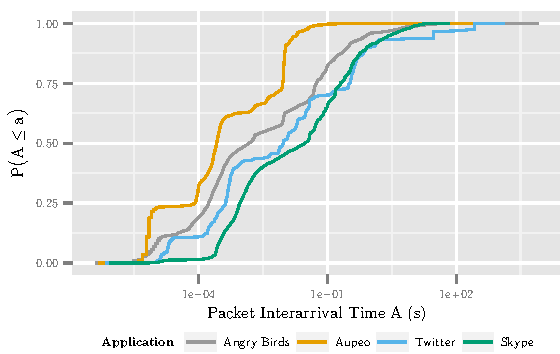
\includegraphics{network/network_traces/numerical_results/figures/interarrival_times}
\caption{CDF of interarrival times for considered applications}\label{fig:network:network_traces:numerical_results:traffic:interarrival_times}
\end{figure}

\begin{table}
  \centering
  \caption{Mean and standard deviation of interarrival time and bandwidth for considered applications}
  \label{tab:network:network_traces:numerical_results:traffic_statistics}
  \begin{tabular}{lcccc}
  	\toprule
    Application&\multicolumn{2}{c}{Interarrival time (\si{\second})}&\multicolumn{2}{c}{Bandwidth (\si{\kilo\bit\per\second})}\\
    \cmidrule(lr){2-3}\cmidrule(lr){4-5}
    &Mean&Standard deviation&Mean&Standard deviation\\
    \midrule
    Angry Birds&0.66 &15.90 & 4.42 & 4.50\\
    Aupeo&0.06 & 3.06& 129.76 & 482.63\\
    Twitter& 8.91&44.09 & 0.27 & 0.04\\
    Skype& 0.55 &1.95 & 1.30 & 1.84\\
    \bottomrule
  \end{tabular}
\end{table}

\paragraph*{Angry Birds}
We see that there are no distinct peaks in interarrival time, which would indicate a periodic behaviour.
Furthermore, we see that \SI{5}{\percent} of all interarrival times are greater than \SI{1}{\second}.
As we consider only \gls{TDCH} values above \SI{1}{\second}, those are candidates for triggering state transitions.
The mean interarrival time is \SI{0.66}{\second}, with a relatively high standard deviation of \SI{15.90}{\second}.
This is caused by the low interarrival times in one advertisement request at the beginning of each new level and the relatively large interarrival times between two advertisements.
Mean bandwidth is relatively low with \SI{4.42}{\kilo\bit\per\second} and a high standard deviation of \SI{4.5}{\kilo\bit\per\second}.
These differences can be explained by considering the behaviour of the application.
During long phases of use no traffic is sent, and after a level is restarted, a new advertisement has to be obtained, causing the transmission of data.
Note that no level data is downloaded during gameplay at all, as the complete game is downloaded during the installation process.

\paragraph*{Aupeo}
We see that the application generates packets with relatively small interarrival times with a small mean interarrival time of \SI{0.06}{\second}.
The high standard deviation of \SI{3.06}{\second} is caused by the wait between two tracks.
Furthermore, we see a high mean bandwidth of \SI{129.76}{\kilo\bit\per\second}, and a standard deviation of \SI{482.63}{\kilo\bit\per\second}.
This is caused by the difference in traffic activity between times when tracks are either downloaded or not.

\paragraph*{Twitter}
We see that \SI{90}{\percent} of all transmissions occur with an interarrival time of less than \SI{1}{\second}.
Also, we can observe a high mean interarrival time of \SI{8.91}{\second} and a high standard deviation of \SI{44.49}{\second}.
Additionally, the mean bandwidth is low with only \SI{0.27}{\kilo\bit\per\second} and a low standard deviation of \SI{0.04}{\kilo\bit\per\second} due to the fact that Twitter text messages are only \(140\) characters in length and thus only a low volume of traffic needs to be transmitted.

\paragraph*{Skype}
Similar to the Twitter application, we see that \SI{90}{\%} of all packets occur with an interarrival time of less than \SI{1}{\second}.
However, in contrast to Twitter, we see a low mean interarrival time of \SI{0.55}{\second} with a standard deviation of \SI{1.95}{\second}.
Further, we observe a relatively low mean bandwidth of \SI{1.30}{\kilo\bit\per\second} and a standard deviation of \SI{1.8}{\kilo\bit\per\second}.

\begin{figure}
\centering
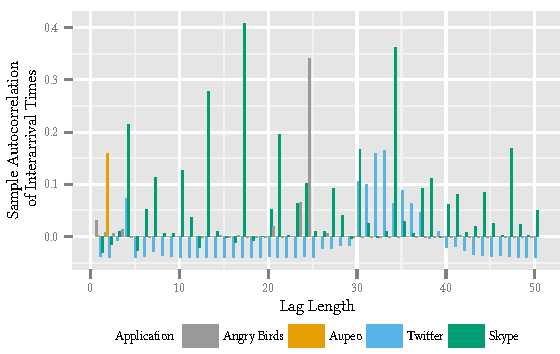
\includegraphics{network/network_traces/numerical_results/figures/autocorrelation}
\caption{Autocorrelation of interarrival times for considered applications}\label{fig:network:network_traces:numerical_results:traffic:autocorrelation}
\end{figure}

To further study the traffic patterns of the applications, we study the autocorrelation of the packet interarrival time with regard to the lag length in \reffig{fig:network:network_traces:numerical_results:traffic:autocorrelation}.
We note that all studied applications present completely different autocorrelations for the interarrival times.
This is one of the reasons that the applications under consideration will display different signalling behaviour in the next section.

\subsubsection*{Influence of Application Characteristics on Optimisation with Network Timers}\label{sec:network:network_traces:numerical_results:application_influence}
This section studies the impact of traffic generated by applications on both the network and the
\gls{QoE} of the user.
We consider two metrics.
First, we consider the frequency of signalling messages induced at network components such as an \gls{RNC}.
In light of network outages caused by so called signalling storms, a large number of signalling messages leading to overload at network equipment, it is in the interest of a network operator to reduce the number of signalling messages arriving at the \gls{RNC}.
One possible way to reduce the signalling frequency \gls{SF} is to modify network timer values, i.e., \gls{TDCH} and \gls{TFACH}.

As discussed in \refsec{sec:network:background:energy_consumption_qoe}, the \gls{QoE} a user perceives while using his device is influenced by the battery life of the \gls{UE}.
Thus, the second metric considered is the device’s power drain which is influenced by the used network model and associated timer settings.
As described in \refsec{sec:network:network_traces:calculating_metrics}, based on a measurement trace for an application we use \refalg{alg:network:network_traces:performance_evaluation:inferring_network_state:inference_algorithm} to infer the state transitions occurring during the use of the application.
Then, we calculate the relative time spent in each state and use \reftab{tab:network:network_traces:calculating_metrics:power_consumption} to compute the mean power
drain of the radio interface during the measurement.
We study both metrics, first on its own and then aggregated for both network models introduced in \refsec{sec:network:background:umts_rrc}.

In this section we first consider the Three State Model, which describes the default behaviour in \gls{3G} networks. 
Then, we describe the influence of the Two State Model which models a network behaviour similar to that if proprietary fast dormancy algorithms are used.
These algorithms have been identified as one of the causes of a signalling storm~\cite{NSN2011}.
Finally, we summarize the results and discuss the possible ramifications of using network timer values to reduce the signalling frequency.

\paragraph*{Three State Model: Signalling Frequency vs. Power Consumption}\label{sec:network:network_traces:numerical_results:three_states}
First, we investigate the signalling frequency generated by the studied applications for the three state network model. 
\reffig{fig:network:network_traces:numerical_results:three_states:three_states:signalling} shows the signalling frequency \gls{SF} with regard to the \gls{TDCH} timer.
\begin{figure}
	\centering
	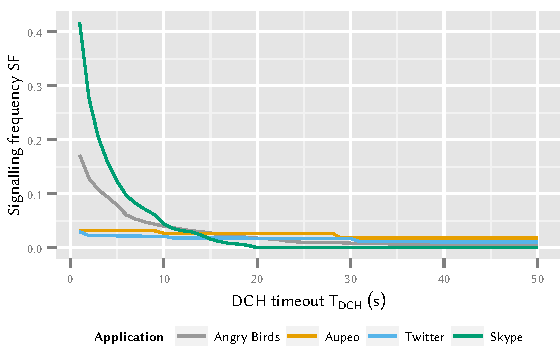
\includegraphics{network/network_traces/numerical_results/figures/3_state_tdch_vs_frequency}
	\caption{Signalling Frequency \gls{SF} for varying \gls{TDCH} timers for the Three State Model}\label{fig:network:network_traces:numerical_results:three_states:three_states:signalling}
\end{figure}
For all studies of the Three State Model, the \gls{TFACH} timeout is set to \(\gls{TFACH} = 2\cdot  \gls{TDCH}\), a realistic value as shown in \cite{Qian2011}.
We see that for \gls{TDCH} timers shorter than \SI{6}{\second} the Skype application in \gls{RRC_idle} mode generates the highest signalling frequency.
The Angry Birds application generates the second highest frequency of signalling messages, followed by the Aupeo application.
The Twitter application generates the smallest signalling frequency.
If the \gls{TDCH} value is longer than \SI{15}{\second}, this order changes.
However, in general the signalling frequency for higher \gls{TDCH} timeouts is lower than for shorter \gls{TDCH} timeouts.
Now, the Aupeo application has the highest signalling frequency, followed by the Twitter application.
The signalling frequency for the Angry Birds application takes the third place.
The application which generated the highest signalling frequency generates the lowest frequency for higher timeout values.
This behaviour can be explained by the fact that the Skype application sends keep-alive messages with an interval of less than \SI{20}{\second}.
If the timer is greater than the interval time of the keep-alive messages, the \gls{UE} stays always connected and thus generates almost no signalling.

These results show that the traffic patterns of the application have a large influence on the generated signalling frequency.
Signalling is generated for every pause in sending or receiving larger than the configured timeouts.
If such pauses occur frequently, this increases the signalling frequency as shown on the examples of Skype and Angry Birds.
Applications with more time between the sending or receiving of data cause less signalling, as shown by Aupeo and Twitter.
Furthermore, we can observe that the signalling frequency can be reduced by increasing the \gls{TDCH} timeout, with the minimum being reached as \gls{TDCH} approaches infinity.
From a signalling frequency perspective, a value of \SI{20}{\second} would probably be sufficient, however if other metrics such as radio resource consumption are considered \SI{10}{\second} would be acceptable for a network operator.

Based on this finding, we see that increasing the \gls{TDCH} timer decreases the signalling frequency \gls{SF} at the \gls{RNC}.
However, the actual signalling frequency depends on the application running at the \gls{UE}.
From a network operator's point of view, the Three State Model should always be preferred to the Two State Model because it generates less signalling messages per second, thus decreasing the load at the \gls{RNC}.
This view does however not consider the additional radio resources which are kept in use for a longer time if larger \gls{TDCH} values are used.
Additionally, it should be noted that the choice of the network model is sometimes outside of the domain of the network operator.
Proprietary Fast Dormancy algorithms, as the considered Two State Model, are enabled on the \gls{UE} by the user.

\begin{figure}
	\centering
	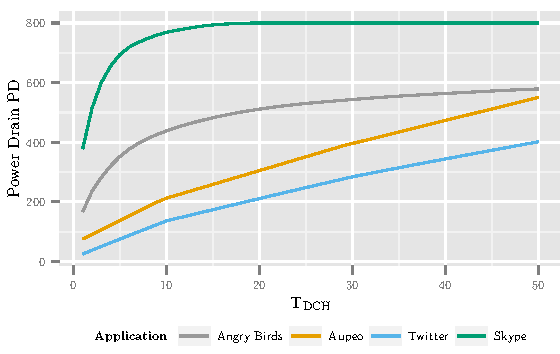
\includegraphics{network/network_traces/numerical_results/figures/3_state_tdch_vs_power_drain}
	\caption{Power Drain \gls{PD} for varying \gls{TDCH} timers for the Three State Model}\label{fig:network:network_traces:numerical_results:three_states:power_drain}
\end{figure}
In \reffig{fig:network:network_traces:numerical_results:three_states:power_drain} we consider the power drain if the network uses the Three State Model, i.e. if the Fast Dormancy mode of the \gls{UE} is disabled.
The figure shows the mean power drain \gls{PD} of the device with regard to the \gls{TDCH} timeout.
Possible values range between \SI{0}{\milli\watt} if the \gls{UE} was in \gls{RRC_idle} state during the whole measurement and \SI{800}{\milli\watt} if the \gls{UE} was in \gls{RRC_DCH} state during the complete measurement.
We see that the least power over all considered \gls{TDCH} values is consumed by the Twitter application.
The second least power drain is required by Aupeo, followed by Angry Birds.
Finally, the most power is consumed by Skype.
Here we see that the maximum value of \SI{800}{\milli\watt} is reached at a \gls{TDCH} timeout of \SI{20}{\second}.
This is because, due to the periodic traffic behaviour of Skype, the device is always in \gls{RRC_DCH} state.
Again, we see that the traffic characteristics of the applications impact the power drain.
Applications with more network activity are forced to stay in more power consuming states for a longer time.
We see that for very small network timers, the power drain is minimal.
However, as seen in the last section small timers increase the signalling frequency at the \gls{RNC}.
Again, a choice of \SI{10}{\second} for the \gls{TDCH} timer can be seen as a compromise between signalling frequency \gls{SF} and power drain \gls{PD}.

\begin{figure}
	\centering
	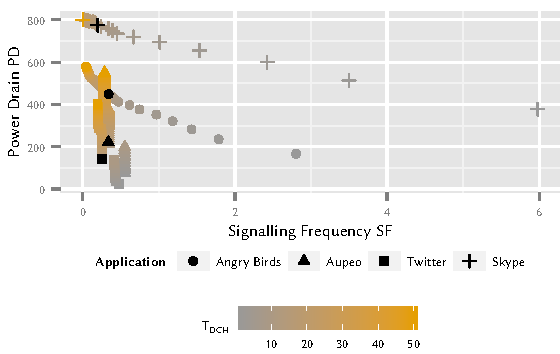
\includegraphics{network/network_traces/numerical_results/figures/3_state_signalling_vs_power_consumption}
	\caption{Influence of manipulating \gls{TDCH} timer on Signalling Frequency \gls{SF} and Power Drain \gls{PD} for the Three State Model. Filled marker highlights \(\gls{TDCH} = \SI{11}{\second}\)}\label{fig:network:network_traces:numerical_results:three_states:trade_off}
\end{figure}
Finally, we aggregate both metrics in in \reffig{fig:network:network_traces:numerical_results:three_states:trade_off}.
The X-axis of the figure gives the signalling frequency.
On the Y-axis we show the power drain \gls{PD}.
Different \gls{TDCH} values are shown by different colors as specified by the colorbar.
First, we consider Angry Birds.
We observe that as the signalling frequency approaches zero, the power drain rapidly increases, even if only small gains in signalling frequency reduction can be achieved.
The Aupeo application presents a completely different picture.
Here, we can see multiple almost horizontal lines of markers.
If \gls{TDCH} is chosen in this range, each increase of \gls{TDCH} brings a small decrease in signalling frequency \gls{SF} for a increase in power drain \gls{PD}.
However, some points of discontinuity exist.
If for example the \gls{RRC_DCH} timer is increased from \SI{10}{\second} to \SI{11}{\second}, a decrease in signalling frequency \gls{SF} of \SI{40}{\percent} can be achieved by only suffering from a small increase in power drain.
These points of discontinuity would present themself to be suitable targets of optimisation.
Next, we consider the Twitter application.
It displays a similar behaviour as the Aupeo application, with multiple points of discontinuity.
Note that Twitter exhibits a different point of discontinuity, and the \gls{TDCH} value of \SI{10}{\second}, which provided good results for Aupeo is not optimal for Twitter.
Finally, Skype again shows a completely different picture then all the other considered applications.
First, note that due to the large signalling frequency \gls{SF} of Skype for small values of \gls{TDCH}, \(\gls{TDCH} = \SI{1}{\second}\) is not displayed in the figure.
Furthermore, as the \gls{TDCH} timer increases above \SI{20}{\second} the signalling frequency \gls{SF} does not decrease any further, and the power drain \gls{PD} remains at the maximum value.
We observe that there is no common optimal value for all applications which would result in an acceptable tradeoff.


\paragraph*{Two State Model: Signalling Frequency vs. Power Drain}\label{sec:network:network_traces:numerical_results:two_states}
Now, we study the consequences of the application traffic in a network using the Two State Model.
The Two State Model occurs in reality if Fast Dormancy implementations are considered.
Here, the \gls{UE} disconnects from the network if for a certain time no traffic is sent or received in order to reduce power drain.
\begin{figure}
	\centering
	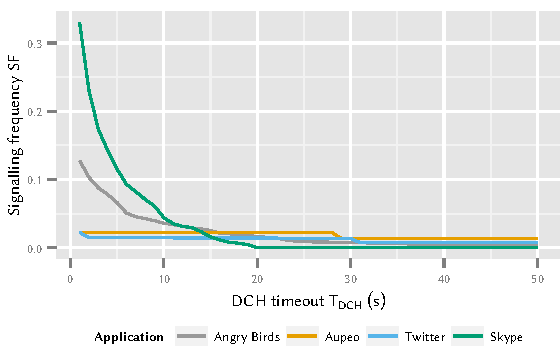
\includegraphics{network/network_traces/numerical_results/figures/2_state_tdch_vs_frequency}
	\caption{Signalling Frequency \gls{SF} for varying \gls{TDCH} timers for the Two State Model}\label{fig:network:network_traces:numerical_results:two_states:signalling}
\end{figure}
As for the Three State Model, \reffig{fig:network:network_traces:numerical_results:two_states:signalling} shows the signalling frequency \gls{SF} with regard to the setting of the \gls{TDCH} timer.
We see the same general behaviour as with the Three State Model, however the signalling frequency generated by each of the applications for the Two State Model are usually higher.
For example, even for relatively high \gls{TDCH} timeout values of \SI{10}{\second}, the Angry Birds application causes \SI{270}{\percent} of the signalling frequency \gls{SF} as in a network using the Three State Model.

\begin{figure}
	\centering
	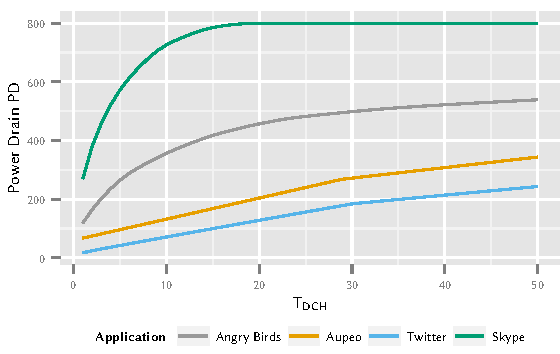
\includegraphics{network/network_traces/numerical_results/figures/2_state_tdch_vs_power_drain}
	\caption{Power Drain \gls{PD} for varying \gls{TDCH} timers for the Two State Model}\label{fig:network:network_traces:numerical_results:two_states:power_drain}
\end{figure}
Next, we consider the changes in the power drain of the \gls{UE} if the user decides to enable Fast Dormancy, i.e. switch to a Two State Model, in \reffig{fig:network:network_traces:numerical_results:two_states:power_drain}.
As with the signalling frequency, we only see a quantitative difference to the Three State Model.
Again, we compare the differences between Two State Model and Three State Model on the example of the Angry Birds application.
For the same considered \gls{TDCH} timeout of \SI{10}{\second}, we see a decrease of \SI{81}{\percent} in power drain \gls{PD} when compared with the Three State Model.

\begin{figure}
	\centering
	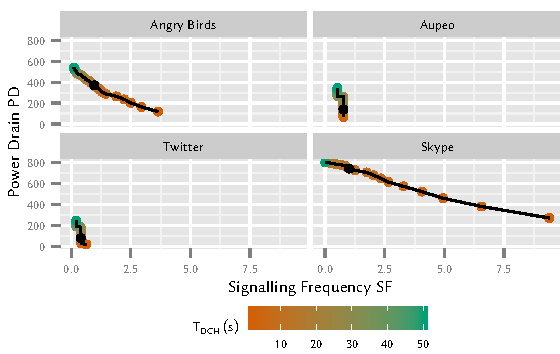
\includegraphics{network/network_traces/numerical_results/figures/2_state_signalling_vs_power_consumption}
	\caption{Influence of manipulating \gls{TDCH} timer on Signalling Frequency \gls{SF} and Power Drain \gls{PD} for the Two State Model. Filled marker highlights \(\gls{TDCH} = \SI{11}{\second}\)}\label{fig:network:network_traces:numerical_results:two_states:trade_off}
\end{figure}
Finally, we compare the influence of changes of thr \gls{TDCH} timeout on both signalling frequency \gls{SF} and power drain \gls{PD} for the Two State Model in \reffig{fig:network:network_traces:numerical_results:two_states:trade_off}.
As for the Three State Model, we see that there is no tradeoff between power drain and signalling frequency which would be acceptable for all application.
Even for single applications \gls{TDCH} values such as \SI{10}{\second} which was an acceptable tradeoff Angry Birds is no longer a good choice in the Two State Model.

\subsubsection*{Consequences of Trade-Off: Signalling Frequency vs. Power Consumption}\label{sec:network:network_traces:numerical_results:trade_off}

In order to illustrate the impact of the behaviour discussed in the previous section, we compare the influence of the \gls{TDCH} timer on an application with different traffic characteristics, for example the Aupeo application as shown in \reffig{fig:network:network_traces:numerical_results:consequences:aupeo}.
\begin{figure}
	\begin{subfigure}[b]{.5\textwidth}
	\centering
	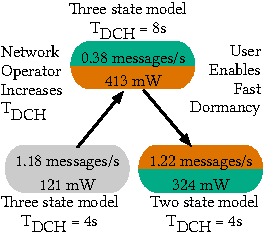
\includegraphics{network/network_traces/numerical_results/figures/consequences_angry_birds}
	\caption{Angry Birds}\label{fig:network:network_traces:numerical_results:consequences:angry_birds}
	\end{subfigure} 
	\begin{subfigure}[b]{.5\textwidth}
	\centering
	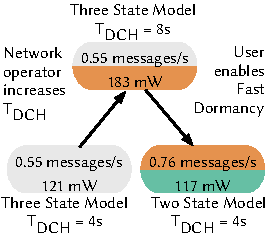
\includegraphics{network/network_traces/numerical_results/figures/consequences_aupeo}
	\caption{Aupeo}\label{fig:network:network_traces:numerical_results:consequences:aupeo}
	\end{subfigure}

	\caption{Influence of manipulating \gls{TDCH} timer on different applications}\label{fig:network:network_traces:numerical_results:consequences}
\end{figure}
The signalling frequency \gls{SF} before the increase of the \gls{TDCH} timer was \(0.55\) messages per second, after the change to \(\gls{TDCH} = \SI{8}{\second}\) the signalling frequency remains unchanged.
Thus, the policy change based on one application brings no significant gain to other applications.
However, from a user's point of view, the power drain \gls{PD} increased from \SI{121}{\milli\watt} to \SI{183}{\milli\watt}.
Again, we assume the user activates fast dormancy to deal with the increase in power drain of more than $50\%$.
This results in a decrease of power drain \gls{PD} to \SI{117}{\milli\watt}, and an increase of overall signalling frequency \gls{SF} to \(0.76\) messages per second.
By changing the value without considering all applications, the network operator has decreased the \gls{QoE} for other users, and worsened his overall situation.
Thus, due to the large number of applications it seems impossible to optimise the \gls{TDCH} timeout to reduce the signalling frequency without negatively impacting the users \gls{QoE} in unexpected ways.

There exist applications, like Twitter and Aupeo, where optimisation by modifying the \gls{TDCH} values can provide acceptable results.
However, these optimisations are only successful if a single application or network model is considered.
For other applications, like Angry Birds or Skype, this optimisation approach does not seem to be successful.
A reduction of signalling frequency and power drain is possible, if the application developers are incentivised to optimise their applications in these regards.
In \cite{Qian2011} the authors suggest methods to achieve this optimisation, for example batch transfer of advertisements for applications like Angry Birds or decreasing the refresh rate in applications like Skype.
However, at the moment application developers are neither receiving incentives to optimise applications in this way, nor do hardware vendors provide interfaces to facilitate such optimisation.
Such interfaces would allow application developers to schedule their data transmissions in such a way that both signalling and battery drain would be reduced.
Additionally, these interfaces would need to allow the application developer to specify whether sending the transmission is urgent.
One example of such urgency would be if the application is being actively used by the user and requires the feedback of the transmission.
If the data is being sent as a regular update while the application is running in the background it could be scheduled for later transmission as suggested by \cite{calder2010, vergara2012}.

\subsection{Influence of Network Configuration and Background Traffic on Web QoE}\label{sec:network:network_traces:numerical_results:web_qoe}
So far we have discussed only power drain as a \gls{QoE} influence factor.
For applications like web browsing, one relevant QoE influence factor are page load times.
Therefore, we consider a web QoE model which quantifies the impact of page load times on mean opinion scores \cite{egger2012a}.
We distinguish here between \emph{web \gls{QoE}} and \emph{\gls{QoE}}, as no \gls{QoE} models are currently existing which consider page load times as well as power drain.
In this section, we study the impact of background traffic as well as network timer settings on the page load time of an image and the resulting \gls{MOS}.
For this study, we only consider the three state network model, but the results can be applied to the 2-state model as well.

We assume a scenario, where a user is running a background application like Twitter or Skype.
Then, while the application is in the background, the user begins to download an image from a website.
Due to the background traffic, and depending on the network model and associated timer values, the \gls{UE} may be currently either in \gls{RRC_idle}, \gls{RRC_FACH} or \gls{RRC_DCH} state.
We give the probability of a random observer encountering the system in \gls{RRC_FACH} state by \(p_{\gls{RRC_FACH}}\) and the probability of a random observer encountering in \gls{RRC_idle} state by $p_{\gls{RRC_idle}}$.
If the device is currently not in \gls{RRC_DCH} state, it takes some time to connect.
This promotion time depends on the current state and is according to \cite{Qian2010b} \SI{2}{\second} if the \gls{UE} is in \gls{RRC_idle} state and \SI{1.5}{\second} if the device is in \gls{RRC_FACH} state.
For this study, we assume that the user randomly chooses a time to begin downloading an image.
The time until the image is displayed consists of the time to load the page \(t_p\), as well as the time to go online \(t_o\), where \(t_o\) is the mean time to go online, given as 
\[t_o = p_{\gls{RRC_idle}} \cdot \SI{2.5}{\second} + p_{\gls{RRC_FACH}} \cdot \SI{1.5}{\second}.\]
In reality, an additional delay is added due to the latency of the physical display, however as this happens in a smaller timescale we neglect it in this model.
Thus, the total time \(t\) that is required to download the image is given by \(t = t_o + t_p\).

The authors of \cite{egger2012a} give a function to calculate the \gls{MOS} based on the required page load time as \(QoE(t) = a\cdot \ln t + b\), were \(a\) and \(b\) depend on the type of content being downloaded.
For our scenario, picture download, values of \(a = -0.8\) and \(b = 3.77\) are suggested.
It has to be noted that for different web sites, the logarithmic function was still observed, but different values for \(a\) and \(b\) were obtained as given in \cite{egger2012a}.
These values depend for example on the type of web page as well as the size of the content.
Nevertheless, the results presented in this section are therefore generalizable for web browsing to various pages.
This allows us to give an expected \gls{MOS} for downloading pictures while a background application is influencing the probability of a device already being in \gls{RRC_DCH} state or still having to be promoted to \gls{RRC_DCH} state.

\begin{figure}
	\begin{subfigure}[b]{\textwidth}
	\centering
	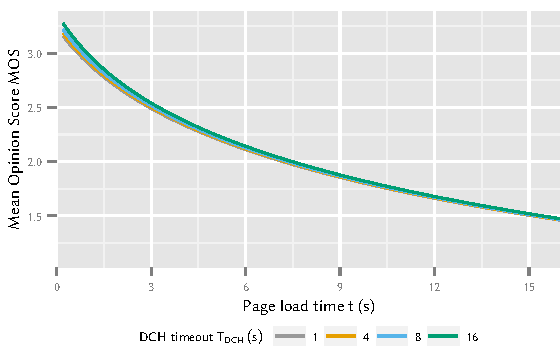
\includegraphics{network/network_traces/numerical_results/figures/qoe_with_backgroundapp_twitter}
	\caption{Background traffic generated by Twitter}\label{fig:network:network_traces:numerical_results:web_qoe:twitter}
	\end{subfigure} 

	\begin{subfigure}[b]{\textwidth}
	\centering
	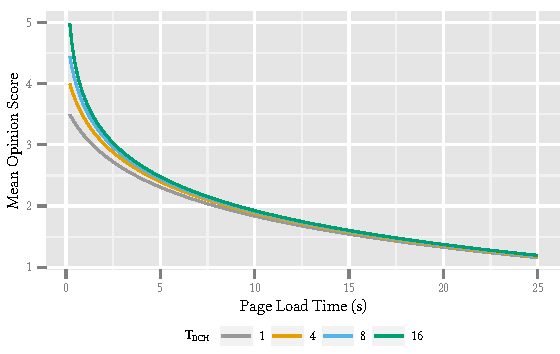
\includegraphics{network/network_traces/numerical_results/figures/qoe_with_backgroundapp_skype}
	\caption{Background traffic generated by Skype}\label{fig:network:network_traces:numerical_results:web_qoe:skype}
	\end{subfigure}

	\caption{Perceived Web-\gls{QoE} for loading a page with existing background traffic}\label{fig:network:network_traces:numerical_results:web_qoe}
\end{figure}

Using this methodology, we study the influence of background traffic on the \gls{QoE} for two background applications with different traffic characteristics.
In \reffig{fig:network:network_traces:numerical_results:web_qoe:twitter} we assume that the user is running the Twitter application as a background process.
The application is set to update the users status feed every \SI{300}{\second}.
In \reffig{fig:network:network_traces:numerical_results:web_qoe:skype} the user is running the Skype application as a background application.
This application sends keep alive messages every \SI{20}{\second}.
For each application, we assume the three state network model with \gls{TDCH} settings of \SIlist{1;4;8;16}{\second}.
We always set \(\gls{TFACH} = 2\cdot \gls{TDCH}\).
In both figures we show the assumed page load time, as provided by the network, on the X-axis for values from \SIrange{0.2}{25}{\second}.
We assume \SI{0.1}{\second} as a lower bound because page load times lower than \SI{0.1}{\second} seconds are not distinguishable \cite{egger2012b} by humans.
The calculated \gls{MOS} values are given on the Y-Axis.

The picture downloads with the background traffic generated by the Twitter application result in \gls{MOS} values beginning at \(3.15\) for \(\gls{TDCH} = \SI{1}{\second}\), \(3.18\) for \(\gls{TDCH} = \SI{4}{\second}\), \(3.21\) for \(\gls{TDCH} = \SI{8}{\second}\), and \(3.27\) for \(\gls{TDCH} = \SI{16}{\second}\) respectively.
With increasing page load time, the \gls{MOS} again decreases.
This behaviour is due to the fact that the Twitter application periodically sends traffic every \SI{300}{\second}.
Then, no further activity occurs until the next refresh occurs.
In this time, the \gls{UE} transitions to \gls{RRC_idle} state.
This traffic characteristic causes a high probability of a user encountering the device in a \gls{RRC_idle} state.
Additionally, the traffic characteristics of the background application show that different \gls{TDCH} settings impact the web \gls{QoE} only marginally, resulting in the lines in the graph being grouped close together.

In contrast, downloading pictures with the Skype application generating background traffic, causes different \gls{MOS} values.
For a page load time of \SI{0.2}{\second} the \gls{MOS} value with \(\gls{TDCH} = \SI{1}{\second}\) is \(3.49\) with \(\gls{TDCH} = \SI{4}{\second}\) we get \(3.99\) for \(\gls{TDCH} = \SI{8}{\second}\) we get a \gls{MOS} value of \(4.44\) and finally for \(\gls{TDCH} = \SI{16}{\second}\) we get \(4.99\) respectively.
For increasing page load times, the \gls{MOS} decreases.
This increased \gls{MOS} values occur because of the high frequency of traffic sent by the Skype application.
Here, every \SI{20}{\second} traffic is sent.
This means that even for relatively low values of \(\gls{TDCH}\) the user has a high probability of encountering a state where no promotion delay is required before the actual page load time can begin.

From these studies we can conclude that, when considering \gls{QoE} on mobile devices, not only the page load time caused by the network but also additional delays caused by the state of the device should be considered.
As shown on two examples, this state can be affected by other applications which are running in the background and generate traffic.



\section{A Performance Model for \glsentryshort{3G} \glsentryshort{RRC} States}\label{sec:network:performance_model}
\cite{Schwartz2013c}

\subsection{System Description and Basic Assumptions}\label{sec:network:performance_model:system_description}

%TODO: Introduction
\newcommand{\PacketIAT}{A}

We consider a \gls{UE} which sends and receives a sequence of data packets via a \gls{3G} \gls{UMTS} network.
As discussed in \refsec{sec:network:background:umts_rrc}, the arrival process of the packet transmissions determines the \gls{RRC} states of the \gls{UE}.
However, the direction of packets, i.e. them originating from the \gls{UE} or the \gls{NodeB}, has no impact on the \gls{RRC} states, as the states depend solely on traffic activity.
Due to the high impact of \gls{RRC} states on traffic patterns, we do not consider packet sizes in this model.
In real \gls{UMTS} networks very small packets might be treated differently for \gls{RRC} states, but we neglect this both for simplicity reasons and because the impact of packet sizes is highly network operator specific~\cite{Qian2010a}.
Furthermore, \gls{RRC} state transitions are complex procedures depending on implementation details of the \gls{UE}, the specific \gls{UMTS} release, and the configurations by the network operator.
In order to keep our model simply, but realistic, we reduce the set of standardized \gls{RRC} states and the state transition triggers in the following ways. 

\begin{figure}
	\begin{subfigure}[b]{.5\textwidth}
	\centering
	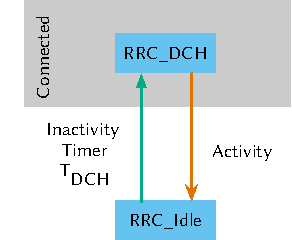
\includegraphics{network/background/figures/two_states}
	\caption{Two State Scenario}\label{fig:network:performance_model:system_description:rrc_state_machines:two_states}
	\end{subfigure}	\begin{subfigure}[b]{.5\textwidth}
	\centering
	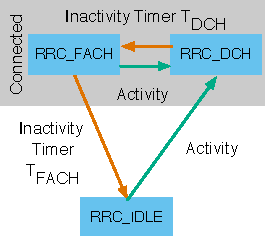
\includegraphics{network/background/figures/three_states}
	\caption{Three State Scenario}\label{fig:network:performance_model:system_description:rrc_state_machines:three_states}
	\end{subfigure}
	\caption{\headershortacr{RRC} State Machine Diagrams}\label{fig:network:performance_model:system_description:rrc_state_machines}
\end{figure}

In a first step we consider only a basic scenario with two \gls{RRC} states: \gls{RRC_idle} and \gls{RRC_DCH} as shown in \reffig{fig:network:performance_model:system_description:rrc_state_machines:two_states}.
The \gls{UE} switches to \gls{RRC_DCH} to transmit or receive data and after an inactivity period of duration \gls{TDCH} it switches back to \gls{RRC_idle}. 
The motivation for the two states \gls{RRC} scenario is twofold.
First, it serves for illustration purposes.
We derive the model step-by-step in this simple scenario to explain the ideas behind the equations.
Then, the ideas can be easily transferred to the more complex three states scenario (cf. \refsec{sec:network:performance_model:system_description:three_states}).
Second, the scenario is of practical relevance since proprietary implementations of the fast dormancy concept \cite{NSN2011} exist, where the \gls{UE} decides to switch to \gls{RRC_idle} shortly after the transmission of a packet without using any other \gls{RRC} state.
Furthermore, this model is very similar to the one found in \gls{LTE} systems.
In \gls{LTE}, only a distinction between connected and disconnected states can be found, which maps to the \gls{RRC_idle} and \gls{RRC_DCH} states discussed in this model.

In our model we aggregate both packets sent and received by the \gls{UE} in in the packet arrival process, which is assumed to be a renewal process, i.e. a process  with identical and independently distributed inter-arrival times, described by the random variable \(\PacketIAT\) as shown in~\reffig{fig:network:performance_model:system_description:rrc_state_machines:two_states}.
Thus, the probability that the time between two consecutive packets is at most \(t\) is \(P(\PacketIAT \leq t) = \PacketIAT(t)\).
We challenge this assumption by studying measurements of packet traces in \refsec{sec:network:performance_model:validations}.

The packet arrivals determine the \gls{RRC} state of the \gls{UE} and the corresponding transitions. Therefore, the packet arrival process can be seen as a modulating process, c.f. \cite{TranGia1983,TranGia1988}, while the state and the signaling process represent modulated, i.e., resulting processes.

\begin{figure}
  \centering
  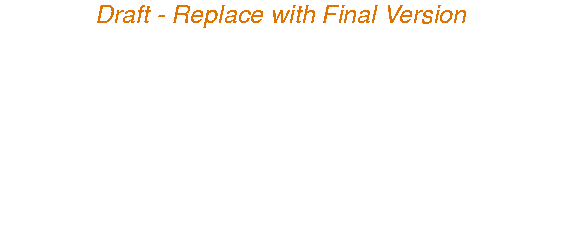
\includegraphics{network/performance_model/system_description/figures/arrival_process}
  \caption{Relation of Packet Arival Process \(\PacketIAT\), State Process, and Signaling Process in the Two State Scenario}
  \label{fig:network:performance_model:system_description:arrival_process}
\end{figure}

\subsubsection*{The Case of Two \headershortacr{RRC} States}\label{sec:network:performance_model:system_description:two_states}

\newcommand{\RRCState}{S}
\newcommand{\PacketIATDensity}{a}
\newcommand{\RRCStateRealization}{s}
\newcommand{\ObservationInterval}{T_{\text{Obs}}}
\newcommand{\ObservationPoint}{t^*}
\newcommand{\ObservationIntervalDensity}{q}
\newcommand{\ObservationIntervalLength}{\tau}
\newcommand{\NormalisationConstant}{c_0}
\newcommand{\NObservedPackets}{n_{\text{P}}}

\paragraph*{State Distribution}
First, we are interested in the state distribution \(P(\RRCState=\RRCStateRealization)\), i.e., the fraction of time the \gls{UE} spends in state \(\RRCStateRealization\in\{\gls{RRC_idle},\gls{RRC_DCH}\}\) for a given inter-packet time \(\PacketIAT\).
For this purpose, we define an observation interval \(\ObservationInterval\), depicted in \reffig{fig:network:performance_model:system_description:arrival_process}, which is assumed to be larger in orders of magnitude than the average packet inter-arrival time \(E[\PacketIAT]\).
In addition, we take the position of an outside observer who observes the state \(\RRCState\) at a random point in time \(\ObservationPoint\), uniformly distributed within the observation interval. 
Then the state distribution \(P(\RRCState=\RRCStateRealization)\) is the probability that the observer encounters the \gls{UE} in state \(\RRCState\) at the time \(\ObservationPoint\). 

We calculate this distribution as 
\begin{equation}
P(\RRCState=\RRCStateRealization)= 
  \int_{0}^\infty \ObservationIntervalDensity(\tau) \cdot 
  P(\RRCState=\RRCStateRealization) \vert \PacketIAT = \ObservationIntervalLength) d\ObservationIntervalLength,
  \label{eq:network:performance_model:system_description:state_distribution} 
\end{equation} 
where \(\ObservationIntervalDensity(\ObservationIntervalLength)\) is the probability density that \(\ObservationPoint\) falls into an interval of length \(\ObservationIntervalLength\) and 
\(P(\RRCState=\RRCStateRealization) \vert \PacketIAT = \ObservationIntervalLength)\)
is the probability that the \gls{UE} is in state \(\RRCState\) under the condition that \(\ObservationPoint\) is within an interval of length \(\ObservationIntervalLength\).

First, we derive \(\ObservationIntervalDensity(\ObservationIntervalLength)\). 
This probability density has to be proportional to \(\PacketIATDensity(\ObservationIntervalLength)\) and to \(\ObservationIntervalLength\), where \(\PacketIATDensity(\ObservationIntervalLength)\) is the probability density function of the random variable \(\PacketIAT\). 
Therefore, we have that 
\(\ObservationIntervalDensity(\ObservationIntervalLength)=\PacketIATDensity(\ObservationIntervalLength)\cdot\ObservationIntervalLength\cdot \NormalisationConstant\)
with the proportionality constant \(\NormalisationConstant\).
Due to 
\(\int_0^\infty \ObservationIntervalDensity(\ObservationIntervalLength)d\ObservationIntervalLength=1\),
we have 
\(\NormalisationConstant=1/E[\PacketIAT]\)
, which leads to
\begin{equation}
\ObservationIntervalDensity(\ObservationIntervalLength)=\frac{a(\ObservationIntervalLength) \cdot \ObservationIntervalLength}{E[\PacketIAT]}.
\label{eq:network:performance_model:system_description:state_distribution:observation_density}
\end{equation}

Next, we derive the conditional probability
\(P(\RRCState=\RRCStateRealization) \vert \PacketIAT = \ObservationIntervalLength)\)
that \(\ObservationPoint\) falls within a period with state \(\RRCState\) under the condition the that the inter-packet time is
\(\PacketIAT = \ObservationIntervalLength)\)
. We use the fact that \(\ObservationPoint\) is uniformly distributed within \(\ObservationIntervalLength\) and calculate the probability 
\(P(\RRCState = \gls{RRC_idle})\)
by considering the relevant cases:
\begin{equation}
P(\RRCState=\gls{RRC_idle}\vert \PacketIAT = \ObservationIntervalLength)=
\begin{cases} 
	0,  & \mbox{if } \ObservationInterval \leq \gls{TDCH} \\ 
    \frac{\ObservationIntervalLength - \gls{TDCH}}{\ObservationIntervalLength}, & \mbox{otherwise.}	 
\end{cases}
\end{equation}

Similarly, we obtain \(P(\RRCState = \gls{RRC_DCH})\) as:
\begin{equation}
P(\RRCState=\gls{RRC_idle} \vert \PacketIAT = \ObservationIntervalLength)=
\begin{cases} 
	1,  & \mbox{if } \ObservationIntervalLength \leq \gls{TDCH} \\ 
    \frac{\gls{TDCH}}{\ObservationIntervalLength}, & \mbox{otherwise.}	 
\end{cases}
\label{eq:network:performance_model:system_description:state_distribution:conditional_probability_dch}
\end{equation} 

\paragraph*{Average Frequency of State Transitions}

\newcommand{\NStateTransitionsIdleToDCH}{n_{\gls{RRC_idle}\rightarrow\gls{RRC_DCH}}}
\newcommand{\NStateTransitionsDCHToIdle}{n_{\gls{RRC_DCH}\rightarrow\gls{RRC_idle}}}
\newcommand{\fStateTransitionsIdleToDCH}{f_{\gls{RRC_idle}\rightarrow\gls{RRC_DCH}}}
\newcommand{\fStateTransitionsDCHToIdle}{f_{\gls{RRC_DCH}\rightarrow\gls{RRC_idle}}}

Next, we estimate the average frequency of state transitions resulting from a given packet arrival process.
For that purpose, we consider again the observation interval \(\ObservationInterval\) and focus on the state transitions from \gls{RRC_idle} to \gls{RRC_DCH} since every switch from \gls{RRC_DCH} to \gls{RRC_idle} results in a switch vice-versa.
The expected number of observed packets during \(\ObservationInterval\) is 
\(E[\NObservedPackets]=\ObservationInterval/E[\PacketIAT]\). 
Furthermore, the probability that time between two consecutive packets exceeds the timer \(\gls{TDCH}\) is
\begin{equation} 
P(\PacketIAT > \gls{TDCH}) = 1 - P(\PacketIAT \leq \gls{TDCH}) = 1 - \PacketIAT(\gls{TDCH}).
\end{equation} 
The number of state transitions \(\NStateTransitionsIdleToDCH\) during \(\ObservationInterval)\) directly corresponds to the number of inter-packet times exceeding \(\gls{TDCH}\) since an active connection is torn down after an inactivity period of \(\gls{TDCH}\).
Thus, the expected number is 
\begin{align}
\begin{split}
E[\NStateTransitionsIdleToDCH] & = E[\NObservedPackets] \cdot P(\PacketIAT > \gls{TDCH})\\
	& = \frac{\ObservationInterval}{E[\PacketIAT]}\cdot (1-\PacketIAT(\gls{TDCH})). 
\end{split}
\end{align} 
Hence, the expected frequency of state transitions is 
\begin{equation}
E[\NStateTransitionsIdleToDCH]=\frac{1-\PacketIAT(\gls{TDCH})}{E[\PacketIAT]}.
\end{equation}
The same holds also for the state transitions from \gls{RRC_DCH} to \gls{RRC_idle} and hence 
\(E[\fStateTransitionsDCHToIdle]=E[\fStateTransitionsDCHToIdle]\)
holds.

\subsubsection*{Extension for Three \headershortacr{RRC} States}\label{sec:network:performance_model:system_description:three_states}
In this section, we consider three states: \gls{RRC_idle}, \gls{RRC_DCH}, and \gls{RRC_FACH}.
Again, we assume that the \gls{UE} switches from \gls{RRC_idle} to \gls{RRC_DCH} whenever it transmits or receives data.
After an inactivity of \(\gls{TDCH}\) the \gls{UE} switches to \gls{RRC_FACH}, and after an additional inactivity of \(\gls{TFACH}\), it switches to \gls{RRC_idle}, as depicted in \reffig{fig:network:performance_model:system_description:rrc_state_machines:three_states}.
This scenario usually occurs when the network controls the \gls{RRC} state of the \gls{UE} without proprietary connection tear-down mechanisms implemented on the \gls{UE}.
In today's network some operator transition the \gls{UE} to a state with a paging channel \texttt{URA\_PCH} instead of the \gls{RRC_idle}, but the resource consumptions in both states are very similar and we therefore neglect the \texttt{URA\_PCH} state for simplicity reasons.

\paragraph*{State Distribution}
The state distribution \(P(\RRCState=\RRCStateRealization)\) for the three states $\RRCStateRealization\in\{\gls{RRC_idle},\gls{RRC_FACH},\gls{RRC_DCH}\}$ can be derived in the same way as for the scenario with two states.
Therefore, we present only the conditional probabilities, which differ from the two state case, and use \refeq{eq:network:performance_model:system_description:state_distribution} for the calculation of the distribution.
First, we consider \(\RRCState=\gls{RRC_idle}\): 
\begin{equation} 
P(\RRCState=\gls{RRC_idle} \vert \PacketIAT = \ObservationIntervalLength) =
\begin{cases} 
	0,  & \mbox{if } \ObservationIntervalLength \leq \gls{TDCH}+\gls{TFACH} \\ 
	\frac{\ObservationIntervalLength - (\gls{TDCH}+\gls{TFACH})}{\ObservationIntervalLength}, 
	    & \mbox{otherwise.}
\end{cases}
\end{equation}
For the case of \(\RRCState=\gls{RRC_FACH}\), we have:
\begin{equation} 
P(\RRCState=\gls{RRC_FACH} \vert \PacketIAT = \ObservationIntervalLength) =
\begin{cases} 
	0,  & \mbox{if } \ObservationIntervalLength \leq \gls{TDCH} \\ 
	\frac{\ObservationIntervalLength - \gls{TDCH}}{\ObservationIntervalLength}, 
	    & \mbox{if }\gls{TDCH}<\ObservationIntervalLength\leq \gls{TDCH}+\gls{TFACH} \\
	\frac{\gls{TFACH}}{\ObservationIntervalLength} 
	    & \mbox{if } \ObservationIntervalLength > \gls{TDCH}+\gls{TFACH} 
\end{cases}
\end{equation}

The probability for the \gls{RRC_DCH} state \(P(\RRCState=\gls{RRC_DCH} \vert \PacketIAT = \ObservationIntervalLength)\) does not differ from the two state scenario, i.e. \refeq{eq:network:performance_model:system_description:state_distribution:conditional_probability_dch}.

\paragraph*{Average Frequency of State Transitions}

\newcommand{\fStateTransitionsDCHToFACH}{f_{\gls{RRC_DCH}\rightarrow\gls{RRC_FACH}}}
\newcommand{\fStateTransitionsFACHToIdle}{f_{\gls{RRC_FACH}\rightarrow\gls{RRC_idle}}}
\newcommand{\fStateTransitionsFACHToDCH}{f_{\gls{RRC_FACH}\rightarrow\gls{RRC_DCH}}}

In contrast to the two state scenario, we have to consider a larger number of state transitions. These are the transitions from \gls{RRC_idle} to \gls{RRC_DCH}, from \gls{RRC_DCH} to \gls{RRC_FACH}, from \gls{RRC_FACH} to \gls{RRC_DCH}, and from \gls{RRC_FACH} to \gls{RRC_idle}.
Other transitions do not occur.
We first calculate the frequency of state transitions from \gls{RRC_DCH} to \gls{RRC_FACH}.
This transition happens every time when the inter-packet time \(\PacketIAT\) exceeds the timer \(\gls{TDCH}\).
Therefore, the derivation is the same as presented above:
\begin{equation}
E[\fStateTransitionsDCHToFACH]=\frac{1-\PacketIAT(\gls{TDCH})}{E[\PacketIAT]}.
\end{equation}
\begin{equation}
E[\fStateTransitionsFACHToIdle]=\frac{1-\PacketIAT(\gls{TDCH}+\gls{TFACH})}{E[\PacketIAT]}.
\end{equation}
Furthermore, all state transitions from \gls{RRC_FACH} to \gls{RRC_idle} correspond to a switch from \gls{RRC_idle} to \gls{RRC_DCH} and therefore 
\(E[\fStateTransitionsIdleToDCH]=E[\fStateTransitionsFACHToIdle].\)
Finally, we calculate \(E[\fStateTransitionsFACHToDCH].\)
These state transitions occur, if \(\gls{TDCH}<\PacketIAT \leq \gls{TDCH}+\gls{TFACH}\).
Therefore, we have 
\begin{equation}
E[\fStateTransitionsFACHToDCH]=\frac{\PacketIAT(\gls{TDCH}+\gls{TFACH})-\PacketIAT(\gls{TDCH})}{E[\PacketIAT]}.
\end{equation}
Other state transitions do not occur in our scenario, as shown in \reffig{fig:network:performance_model:system_description:rrc_state_machines:three_states}).

\subsubsection*{Modeling Signaling Intensity and Power Drain of the \headershortacr{UE}}\label{sec:network:performance_model:system_description:metrics}

\newcommand{\fStateTransitions}{E[f_{ST}]}

We assume that every state transition involves signaling traffic.
In order to quantify signaling load on an abstract level, we define the \gls{SI} of an application, i.e. of a given distribution for \(\PacketIAT\), as the average number of state transitions required for the transmission of a single data packet.
\begin{equation}
\gls{SI} = \frac{\fStateTransitions \cdot \ObservationInterval}{E[\NObservedPackets]}\\
= \fStateTransitions {E[f_{ST}] }\cdot E[\PacketIAT]
\label{eq::sigIntensity}
\end{equation}
where \(\fStateTransitions\) is the sum of all state transitions.
Consequently, \(\gls{SI} \in ]0,2]\) for the two state scenario since every packet can at most cause two state transitions, in the three state scenario \(\gls{SI} \in]0,3]\) holds.
This metric is intended to quantify the relation between transmitted data packets and the involved \gls{RRC} state transitions, which all incur mobile network signaling.
The metric can be extended to capture more details, such as the number and type of signaling messages exchanged for a specific state transition.
Since we will use this metric for more qualitative analysis of source traffic produced by smart-phone applications, we stick to the definition above allowing for an illustrative understanding of the numerical results.

Next, we model the \gls{PD} of the \gls{UE} due to the \gls{UMTS} transmission unit. 
We assume three power levels \()\gls{PD}_{\RRCState}\), one for every state \(\RRCStateRealization\) and calculate the average power drain \(\gls{PD}\) based on the state distribution, which in turn depends on the packet arrival process \(\PacketIAT\).
We obtain
\begin{equation}
\gls{PD} = \sum_{\RRCStateRealization\in\RRCState} \gls{PD}_{\RRCStateRealization} \cdot P(\RRCState=\RRCStateRealization)
\label{eq::powerdrain}
\end{equation}
with \(\RRCState = \{\gls{RRC_idle},\gls{RRC_DCH}\}\) or \(\RRCState = \{\gls{RRC_idle},\gls{RRC_FACH},\gls{RRC_DCH}\}\) depending on wether the two state scenario or the three state scenario is considered.
This is a user-centric metric and gives insights into how efficient the transmission process uses the battery. 
\subsection{Impact of Analytic Traffic Characteristics}\label{sec:network:performance_model:numerical_examples}
First, we validate our performance model by comparing the analytical results with simulations based on measured
packet traces of two real smartphone applications .
Then, we investigate the impact of traffic patterns on signalling load and power drain and derive high-level implications of the model.

\subsubsection*{Model Validations}\label{sec:network:performance_model:validations}

In order to assess the applicability of our performance model, we first have to check whether real-world application traces can be modeled as renewal process, which was our main assumption for the model.
We use the Lewis-Robinson-Test \cite{Ascher1984}, which is a hypothesis test with null hypothesis \(H_0\) that the tested process is a renewal process.
To this end, we use exemplary the measurement, obtained with the measurement testbed introduced in \refsec{sec:network:network_traces:performance_evaluation:measurement}, for two different types of applications: \emph{Twitter} and \emph{K9-Mail}.
According to this test, the null hypothesis cannot be rejected for both of our packet traces at a significance level of \SI{95}{\percent}.
Although this assumption may not be true for all applications, our results show that at least the considered applications can be modeled as a renewal process.

Next, we compare our analytical performance results with \gls{RRC} protocol simulations using measured application and \gls{TCP} traces which are described in more detail in \refsec{sec:network:network_traces:numerical_results:traffic_characterization}.
In order to produce analytical results that correspond to the real applications, we extract the empirical distributions of the inter-packet time \(\PacketIAT\) from the traces for both applications and use these distributions as input for \refeq{eq:network:performance_model:system_description:state_distribution:observation_density}. 

In \reffig{fig:network:performance_model:numerical_examples:validations:analytic_vs_simulation} we compare the accuracy of the results  obtained by the presented method to the values obtained from simulations for the two measured applications and both considered metrics.
We observe that the accuracy for both power drain \(\gls{PD}\) and \(\gls{SI}\) is very high.
In \reffig{fig:network:performance_model:numerical_examples:validations:analytic_vs_simulation:signalling_intensity} the results for both the Mail and Twitter application obtained by the model completely align with the signalling intensity obtained by the simulation.
The comparison of analytical results for the power drain to the simulation in \reffig{fig:network:performance_model:numerical_examples:validations:analytic_vs_simulation:power_drain} leads to the same conclusions as for the signalling intensity.

\begin{figure}
	\begin{subfigure}[b]{\textwidth}
	\centering
	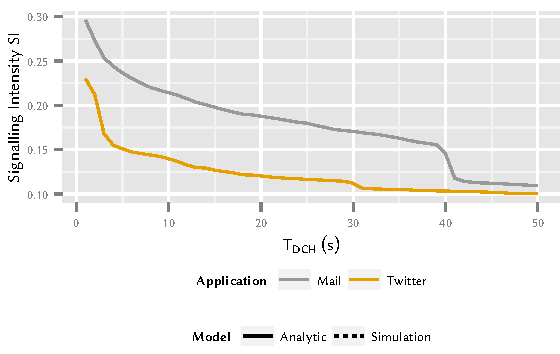
\includegraphics{network/performance_model/numerical_examples/figures/3state_tdch_si_analytic_simulative}
	\caption{Signalling intensity}\label{fig:network:performance_model:numerical_examples:validations:analytic_vs_simulation:signalling_intensity}
	\end{subfigure}

	\begin{subfigure}[b]{\textwidth}
	\centering
	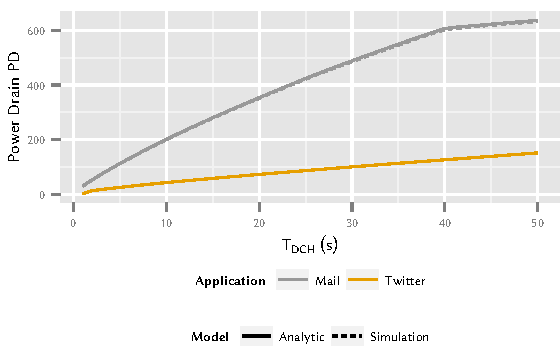
\includegraphics{network/performance_model/numerical_examples/figures/3state_tdch_pd_analytic_simulative}
	\caption{Power drain}\label{fig:network:performance_model:numerical_examples:validations:analytic_vs_simulation:power_drain}
	\end{subfigure}

	\caption{Comparison of the performance model with a \headershortacr{3G} simulation for the Three State Scenario. Lines overlap due to good fit.}\label{fig:network:performance_model:numerical_examples:validations:analytic_vs_simulation}
\end{figure}

\subsubsection*{Impact of Traffic Patterns on Signalling Intensity}\label{sec:network:performance_model:signalling_intensity}
First, we focus on the signalling intensity \(\gls{SI}\) of traffic patterns and check the impact of the average inter-packet time \(E[\PacketIAT]\) and the timer configuration. The signalling intensity \(\gls{SI}\), i.e., the average number of state transitions required for the transmission of a single packet, is an abstract measure for the signalling load produced by a specific traffic pattern.

\paragraph*{Impact of the Average Inter-Packet Time \(E[\PacketIAT]\)}\label{sec:network:performance_model:signalling_intensity:ea}
Some applications, for example those downloading or streaming of videos, send and receive large amounts of data within short time frames.
In contrast, other applications, e.g. social network clients send and receive small amounts of data every few minutes over the time span of some hours or days.

In this section we study the impact of average inter-packet times \(E[\PacketIAT]\) and the burstiness of the traffic pattern, i.e., the coefficient of variation 
\[c_{\PacketIAT} = \frac{\sqrt{\mathrm{Var}[\PacketIAT]}}{\mathrm{E}[\PacketIAT]}\]
 on the signalling load.
For that purpose, we use the simple Two State Model, set the timer \(\gls{TDCH}=\SI{10}{\second}\), consider only the first and the second moment of the inter-packet time \(\PacketIAT\), and assume that \(\PacketIAT\) follows a log-normal distribution, where both moments can be varied independently.

\begin{figure}
	\centering
	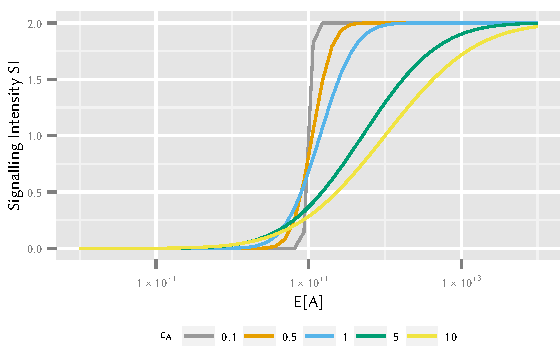
\includegraphics{network/performance_model/numerical_examples/figures/2state_ea_si}
	\caption{Signalling intensity \gls{SI} for different traffic patterns considering the Two State Model with \(\headershortacr{TDCH}=\SI{10}{\second}\) for different traffic patterns.}
	\label{fig:network:performance_model:numerical_examples:validations:analytic_vs_simulation:2state_ea_si}
\end{figure}

In \reffig{fig:network:performance_model:numerical_examples:validations:analytic_vs_simulation:2state_ea_si}, we vary the average inter-packet time \(E[\PacketIAT]\) in six orders of magnitude and investigate the resulting signalling intensity \(\gls{SI}\) for different coefficients of variation \(c_{\PacketIAT}\).
We observe that \(c_{\PacketIAT}\) has no impact on \(\gls{SI}\) for very small inter-packet times \(E[\PacketIAT]<\SI{1e-1}{\second}\).
Here, the \gls{UE} stays in state \gls{RRC_DCH} for the complete time since no inter-packet times \(\PacketIAT>\gls{TDCH}\) occur.
In addition, the impact of \(c_{\PacketIAT}\) is small for very large values of \(E[\PacketIAT]>\SI{1e3}{\second}\).
In this case, the \gls{UE} switches to state \gls{RRC_DCH} and back to state \gls{RRC_idle} for the transmission of every packet. Therefore, the signalling intensity \(\gls{SI}\) approaches the value 2.
For values in between these two extremes, the coefficient of variation \(c_{\PacketIAT}\) has a considerable impact on the signalling intensity \(\gls{SI}\).
More periodic traffic, i.e. smaller values of \(c_{\PacketIAT}\), results in an increase of \(\gls{SI}\) from 0 to 2 very sharp at the value \(E[\PacketIAT]=\gls{TDCH}\), while this increase is more smooth for larger values of \(c_{\PacketIAT}\).
This is due to the fact that for nearly periodic traffic it is crucial whether the timer value \(\gls{TDCH}\) is smaller or larger than \(E[\PacketIAT]\). 
For larger values of \(c_{\PacketIAT}\) this dependency is weaker.

\paragraph*{Impact of the Coefficient of Variation of the Inter-Packet Time \(c_\PacketIAT\)}

Next, we focus on the impact of the timer value \(\gls{TDCH}\) with respect to the burstiness of the traffic.
We use the same setting as before, but fix the average inter-packet time \(E[\PacketIAT]=\SI{4}{\second}\).
While there are differences in \(E[\PacketIAT]\) among users in real world settings, measurement studies have revealed that across all users \(\SI{95}{\percent}\) of the packets are received or transmitted within \(\SI{4.5}{\second}\) of the previous packet \cite{Falaki2010a}.
Therefore, the order of magnitude of \(E[\PacketIAT]=\SI{4}{\second}\) is of practical relevance. 

\begin{figure}
	\centering
	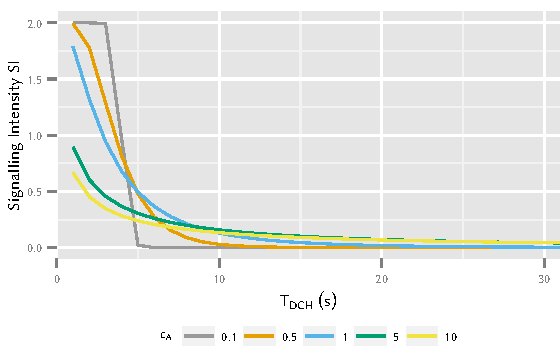
\includegraphics{network/performance_model/numerical_examples/figures/2state_tdch_si}
	\caption{Signalling intensity \(\headershortacr{SI}\) for the Two State Model w.r.t. different timeout values \(\headershortacr{TDCH}\) and coefficient of variations \(c_{\PacketIAT}\).}
	\label{fig:network:performance_model:numerical_examples:validations:analytic_vs_simulation:2state_tdch_si}
\end{figure}


The signalling intensity \(\gls{SI}\) is shown in \reffig{fig:network:performance_model:numerical_examples:validations:analytic_vs_simulation:2state_tdch_si} with respect to the timer value \(\gls{TDCH}\) and the burstiness \(c_{\PacketIAT}\) of the traffic pattern.
Obviously, larger timers lead to less frequent state transitions and therefore to less signalling load.
We observe in addition that the impact of the timer is crucial for nearly periodic traffic.
If the average inter-packet time for nearly periodic traffic is larger than the timer, then every packet transmission involves a state transitions from \gls{RRC_idle} to \gls{RRC_DCH} and a transition back.
In contrast, no transitions are required if the average inter-packet time is shorter than the timer.
With increasing values of \(c_{\PacketIAT}\) the impact of the timer is reduced.
This means that for bursty traffic patterns the timer value is of less importance with respect to the generated signalling load.

\subsubsection*{Impact of Traffic Patterns on Power Drain of the \headershortacr{UE}}\label{sec:network:performance_model:power_drain}
In this section we study the impact of the traffic patterns on the power drain \(\gls{PD}\) of the \gls{UE}.
This metric quantifies how resource-efficient specific traffic patterns and timer configurations are for the battery of the \gls{UE}.

\begin{figure}
	\centering
	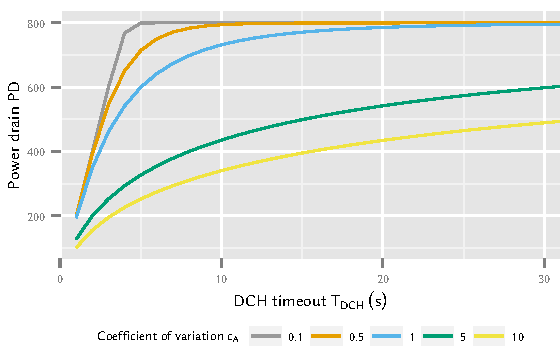
\includegraphics{network/performance_model/numerical_examples/figures/2state_tdch_pd}
	\caption{Power drain \(\headershortacr{PD}\) for the Two State Model w.r.t. different timeout values \(\headershortacr{TDCH}\) and coefficient of variations \(c_{\PacketIAT}\).}
	\label{fig:network:performance_model:numerical_examples:validations:analytic_vs_simulation:2state_tdch_pd}
\end{figure}

For the power drain in the different \gls{RRC} states, we use the same radio network power drain  used in \refsec{sec:network:network_traces:calculating_metrics}.
We investigate the impact of the average inter-packet time, the impact of the timer configuration and validate our model with simulations. 
In \refsec{sec:network:performance_model:signalling_intensity:ea} we have seen that no state transitions occur for very small and very large average inter-packet times \(E[\PacketIAT]\).
This was due to the fact that for very small values the \gls{UE} is continuously in state \gls{RRC_idle} and for large values it switches to state \gls{RRC_DCH} for every packet.
Thus, traffic patterns with very small and very large inter-packet times \(E[\PacketIAT]\) have also no impact on the power drain of the \gls{UE} regardless of the burstyness represented by the coefficient of variation \(c_{\PacketIAT}\).

To study the impact of the timer configuration \(\gls{TDCH}\), we use the same setting as for the signalling load: log-normal distribution of inter-packet time \(\PacketIAT\), \(E[\PacketIAT] = \SI{4}{\second}\) in the Two State Model.
The numerical values shown in \reffig{fig:network:performance_model:numerical_examples:validations:analytic_vs_simulation:2state_tdch_pd} indicate that longer timeouts lead to a higher power drain \(\gls{PD}\).
This is reasonable since the UE stays longer in the power intensive \gls{RRC_DCH} state in these cases.
However, we observe that the burstiness of the traffic pattern has also a considerable impact on the power drain \gls{PD}. 
For example, for \(\gls{TDCH} = \SI{15}{\second}\), the power drain is only \(\SI{400}{\milli\watt}\) for very bursty traffic with \(c_{\PacketIAT} = 10\), while it is almost \(\SI{400}{\milli\watt}\) for less bursty traffic with a \(c_{\PacketIAT} = 1\). 
The reason is that bursty traffic patterns send a lot of traffic during short periods when the UE is in state \gls{RRC_DCH} anyway. During the following off-periods that \gls{UE} can save power in \gls{RRC_idle} state.
Hence, we conclude that longer timeouts and smaller coefficients of variation \(c_{\PacketIAT} = 1\), i.e. more periodic and less bursty traffic, result in a higher power drain of the \gls{UE}.

\subsubsection*{Tradeoff: Energy Consumption vs. Signalling Load}\label{sec:network:performance_model:trade_off}
In \reffig{fig:network:performance_model:numerical_examples:validations:analytic_vs_simulation:2state_pd_vs_si_vs_tdch}, we show the effect of network parameter optimisation using the timer \gls{TDCH} on traffic patterns with varying coefficient of variation.

\begin{figure}
	\centering
	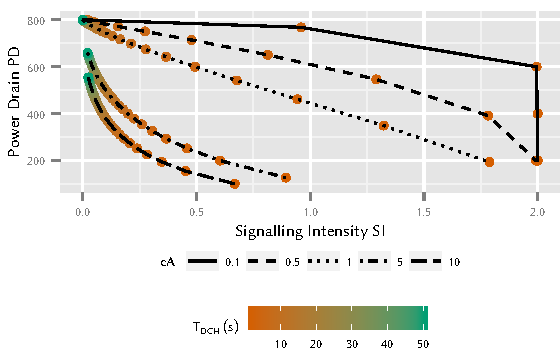
\includegraphics{network/performance_model/numerical_examples/figures/2state_pd_vs_si_vs_tdch}
	\caption{Trade-off between \(\headershortacr{PD}\) and \headershortacr{SI} for the Two State Model.}
	\label{fig:network:performance_model:numerical_examples:validations:analytic_vs_simulation:2state_pd_vs_si_vs_tdch}
\end{figure}

We see that optimisations may decrease signalling by large amounts while only having very little impact on power drain for one specific kind of traffic.
The same timer setting could increase the power drain for another kind of traffic while only offering little benefit with regard to the generated signalling intensity.

\section{Lessons Learned}\label{sec:network:lessons_learned}
In this chapter we studied the impact of smartphone application traffic on mobile communication networks.
We considered three stakeholders interacting in the mobile network.
The \emph{mobile network operator} is interested in preventing so called signalling storms, where network components performance is degraded due to high signalling load caused by applications generating network traffic from users' \glspl{UE}.
The \emph{hardware vendor} is interested in satisfying customers by providing a long battery lifetime for the \gls{UE}, i.e. reducing power drain.
The \emph{application developer} is interested in increasing \gls{QoE} for the applications user.
Each of the stakeholders can influence the mobile network, by manipulating the parameters under its control.
The network operator can manipulate \gls{RRC} timers, increasing the time a smartphone stays connected to the network if no data is sent or received, decreasing the number of connections being established or severed and thus the signalling load in the network. 
The hardware vendor can implement proprietary \gls{RRC} protocol extensions, skipping power intensive connection states in order to reduce power drain.
The application developer can shorten update intervals, in order to provide more up to date events and increase \gls{QoE}.
However, each of the parameters under control of the individual stakeholders influence the \glspl{KPI} of the other stakeholders.

This chapter provides a two-pronged approach to analysing the impact of changes by individual stakeholders on the overall network.

First, we provided an algorithm to derive \gls{RRC} state transitions from traffic measurements of already deployed or prototyped applications.
While proprietary mechanisms exist to directly measure \gls{RRC} state transitions, due to the high price they are usually out of reach for application developers, preventing them from evaluating the impact of their applications on the network.
Based on this algorithm we analyse four popular smartphone applications, and find that while it is possible to find a viable tradeoff between signalling load and power drain for single applications, no such tradeoff exists if multiple applications operating in the network at the same time are considered.
For example, for the considered \emph{Twitter} application, increasing the network timer \TDCH from \SI{10}{\second} to \SI{11}{\second} would result in a decrease of signalling by \SI{40}{\percent}, while only resulting in an increase of power drain of \SI{6}{\percent}.
However, if the \emph{Aupeo} application is running in the same network optimised for the Twitter application, this change results in no reduction of signalling load and an increased power drain of \SI{5}{\percent}. 

Furthermore, we show that network timer optimisation, a practice where network operators manipulate \gls{RRC} timers in order to reduce signalling load, incentivises users to enable proprietary fast dormancy algorithms, resulting in a net increase of signalling load.
For example, if a network operator increases the \TDCH network timer from \SI{4}{\second} to \SI{8}{\second}, in order to reduce the signalling frequency caused by the Angry Birds application by \SI{67}{\percent}, this results in an increased power drain at the user's \gls{UE} of \SI{341}{\percent}.
If the user enables the fast dormancy option of the \gls{UE}, the power drain is decreased by \SI{27}{\percent}, however this increases the signalling frequency above the original value before the reconfiguration of the network operator.
%We also show that while longer \gls{RRC} timers may have an adverse effect on power drain due to the smartphone being longer connected to the network, it results in an increase of Web \gls{QoE}, as this results in web pages being able to be loaded faster if the smartphone is already connected to the network.

Second, we propose an analytical model to derive the \glspl{KPI} from analytical or empirical traffic distributions, in order to evaluate the impact of applications that do not yet exist or classes of applications defined by a common traffic characteristics.
Our results show that different access patterns have a considerable impact on the required resources of the mobile phone and the network.
We identified bursty traffic pattern as particularly resource-efficient with respect to power drain and signalling load.
In contrast, nearly periodic traffic is likely to cause signalling overload due to frequent connection re-establishments, especially when the connection timeout is slightly below the inter-packet time.
This can be observed on the example of a \TDCH timer of \SI{10}{\second}.
Here, the coefficient of variation has no impact on the signalling load for very small inter-packet times \(E[\PacketIAT]<\SI{1e-1}{\second}\) or very large inter-packet times \(E[\PacketIAT]>\SI{1e3}{\second}\).
For example, for a mean inter-arrival time of \(E[\PacketIAT] = 11.5\) seconds, an increase of coefficient of variation from \(0.5\) to \(5.0\) can decrease the signalling load by \SI{53}{\percent}.

Concluding from this chapter, we see that in mobile networks many different players, metrics, and tradeoffs exist.
We highlighted one examples of such a tradeoff, i.e. signalling load vs. power drain and discussed the influence of the current optimisation parameters, the network timers, on another.
However, many additional tradeoffs exist.
For example, the mobile operator has to balance the use of radio resources with the number of generated signalling frequencies.
Furthermore, application providers seek to improve the user experience which usually result in a higher frequency of network polls, creating additional signalling traffic.
The high number of tradeoffs and involved actors in this optimisation problem indicate that the current optimisation technique used by operators is no longer sufficient.

Approaches like \emph{Economic Traffic Management}~\cite{spirou2009} or \emph{Design for Tussle}~\cite{trilogy2008} could be applied to find
an acceptable tradeoff for all parties.
In Economic Traffic Management all participating entities share information in order to enable collaboration.
This collaboration allows for a joint optimisation of the tradeoff.
Design for Tussle aims to resolve tussles at run time, instead instead of design time.
This prevents the case that one actor has full control over the optimisation problem, which would likely result in the actor choosing a tradeoff only in its favour, ignoring all other participants.
One example of an actor providing information for another in order to optimise the total system would be \gls{UE} vendor providing interfaces for application developers to use when sending data.
These interfaces would schedule data to be transmitted in such a way that signalling load and power drain would be reduced, if the application’s requirements allow for it.
Until such interfaces exist, application developers could take the effect of the traffic their applications
produce both on the \gls{UE} and the network into account, for example using the algorithms proposed in this chapter. 
